\chapter{Antibiotic trends analytics}
Having obtained a general analytical view on couples of first-time diagnoses and prescriptions, and cross-checking those results with global trends, the research focusses on antibiotic prescriptions to identify changes of patterns.

Defined time frames in limited temporal windows are selected to make a detailed trajectory analysis related to prescriptive appropriateness compared to antibiotic resistance, without going into details of pathologies.

Such analytics are useful for research, highlighting rising health issues alongside the AIFA reports, and to support pharmaceutical companies using the potentiality of healthcare data. Having information about AICs allows to give a new insight not only on ethical matters, but also on the global market trends.

\section{Identifying antibiotics}
Antibiotics, also known as antibacterials, are medications produced by microorganisms that destroy or slow down the growth of bacteria. They include a range of powerful drugs and are used to treat diseases caused by bacteria. 

A doctor can prescribe a broad-spectrum antibiotic to treat a wide range of infections. A narrow-spectrum antibiotic is only effective against a few types of bacteria. In some cases, a healthcare professional may prescribe to prevent rather than treat an infection, as might be the case before surgery. 
 
 ATC codes related to antibiotics divided by class are:
 \begin{itemize}
 	\item A01AB, A02BD, A07A;
 	\item D01, D06, D07C, D09AA, D10AF;
 	\item G01;
 	\item J, the whole class;
 	\item R02AB;
 	\item S01A, S02A, S03A (removing hormones).
 \end{itemize}

\section{Subset extraction}
The first criteria to impose, considering analytics is going to be made on antibiotic prescriptions, is the actual presence of such. This can be reworded by removing all data related to patients who never had a prescription of an ATC code among the ones previously listed.

There are 794 267 patient with at least one antibiotic prescription in the whole time range (2000-2018), whose total prescriptions consist in 114 044 470 tuples. This implies the remaining 200 000$\sim$ patients only have 4m$\sim$ prescriptions, which is probably justified by a healthier physical state.

Since antibiotics patterns are subject to major changes during years, a big amount of data can be dispersive: pharmaceutical companies make analysis only considering 2-3 years, yet for research purposes an intermediate range is the most informative. A good time span is 10 years, considering most recent ones: since 2018 has to be excluded due to incompleteness, 2008-2017 is the final choice.

Progressive data loss has to be considered, imposing additional constraints of completeness and accuracy. The latest version of the used dataset is a subset of the table prescriptions, with the following restrictions:
\begin{itemize}
	\item AIC corresponding to an antibiotic;
	\item Prescription date between 2008-01-01 and 2017-12-31;
	\item Active general practitioners;
	\item Patients with usable information about sex, date of birth and location.
\end{itemize}

The obtained record set is composed by 8 386 057 tuples, each representing a single prescription.

\section{Global statistics}
Global statistics help to have a general overview of the data, aggregating values to identify most impactful changes and the broad behaviour.

\subsection{Average prescriptions}
The average number of prescriptions has been calculated only considering the number of patients with at least one antibiotic prescription from 2008 onwards (670 634). 

Values are calculated using the R functions \texttt{mean} and \texttt{sd}, only considering the number of patients who received at least one prescription in the determined year.

\begin{center}
	\begin{tabular}{|c|c|c|}
		\hline
		Year & Mean & Standard deviation \\
		\hline
		2008 & 2,72 & 2,73 \\
		\hline
		2009 & 2.75 & 2,78 \\
		\hline
		2010 & 2,72 &  2,76 \\
		\hline
		2011 & 2,69 &  2,73 \\
		\hline
		2012 & 2,68 & 2,76 \\
		\hline
		2013 & 2,74 & 2,84 \\
		\hline
		2014 & 2,79 & 2,88 \\
		\hline
		2015 & 2,79 & 2,79 \\
		\hline
		2016 & 2,77 & 2,91 \\
		\hline
		2017 & 2,72 & 2,84 \\
		\hline
	\end{tabular}
\end{center}

Values show the mean tends to slowly increase, and although there are patients getting up to 30 antibiotic prescriptions each month, the standard deviation is low: the mode both for year and month is 1, so lower values weigh more.

Statistics related to the number of patients with only one antibiotic prescription, making statistics comparing time spans between 2008-2017:
\begin{center}
	\begin{tabular}{|c|c|c|}
		\hline
		Interval & Mean & Standard deviation \\
		\hline
		Year & 118 301,4 & 2 831,65 \\
		\hline
		Month & 40 130,83 & 6 004,2 \\
		\hline
	\end{tabular}
\end{center}

\subsection{Yearly prescriptions}
The number of yearly antibiotic prescriptions is:
\begin{table}[!htb]
	\centering
	\parbox{0.25\textwidth}{
		\begin{footnotesize}
			\begin{tabular}{|c|c|}
				\hline
				Year & Antibiotics \\
				\hline
				2008 & 813 337 \\
				\hline
				2009 & 846 067 \\
				\hline
				2010 & 797 472 \\
				\hline
				2011 & 777 582 \\
				\hline
				2012 & 760 280 \\
				\hline
				2013 & 798 320 \\
				\hline
				2014 & 812 594 \\
				\hline
				2015 & 802 323 \\
				\hline
				2016 & 776 756 \\
				\hline
				2017 & 727 723 \\
				\hline
			\end{tabular}
		\end{footnotesize}
	}
	\qquad
	\begin{minipage}[c]{0.6\textwidth}
		\centering
		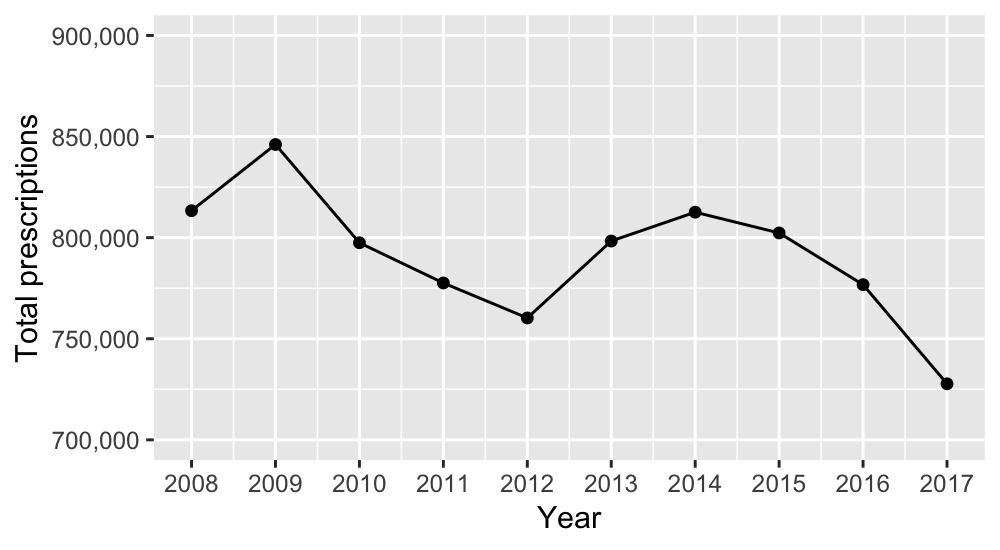
\includegraphics[width=1\textwidth]{../plots/yearly_prescriptions.png}
	\end{minipage}
\end{table}

The 2012 fall might be caused by the substantial decrease of the approved antibiotics by AIFA\cite{calo}, but is noticeable that the number rises starting from 2013 due to antibiotic resistance. 

\subsection{Number of prescriptions trends}
A barplot is the most informative way to visualise trending of number of prescriptions and highlight seasonality. For each month, the amount of patients having the number of prescriptions stated in the x-axis is plotted, using a logarithmic scale.

The scale has been adopted to standardise the quantity of patients having a smaller number of prescriptions (1-2), giving higher bars to larger values.

\begin{figure}[h]
	\centering
	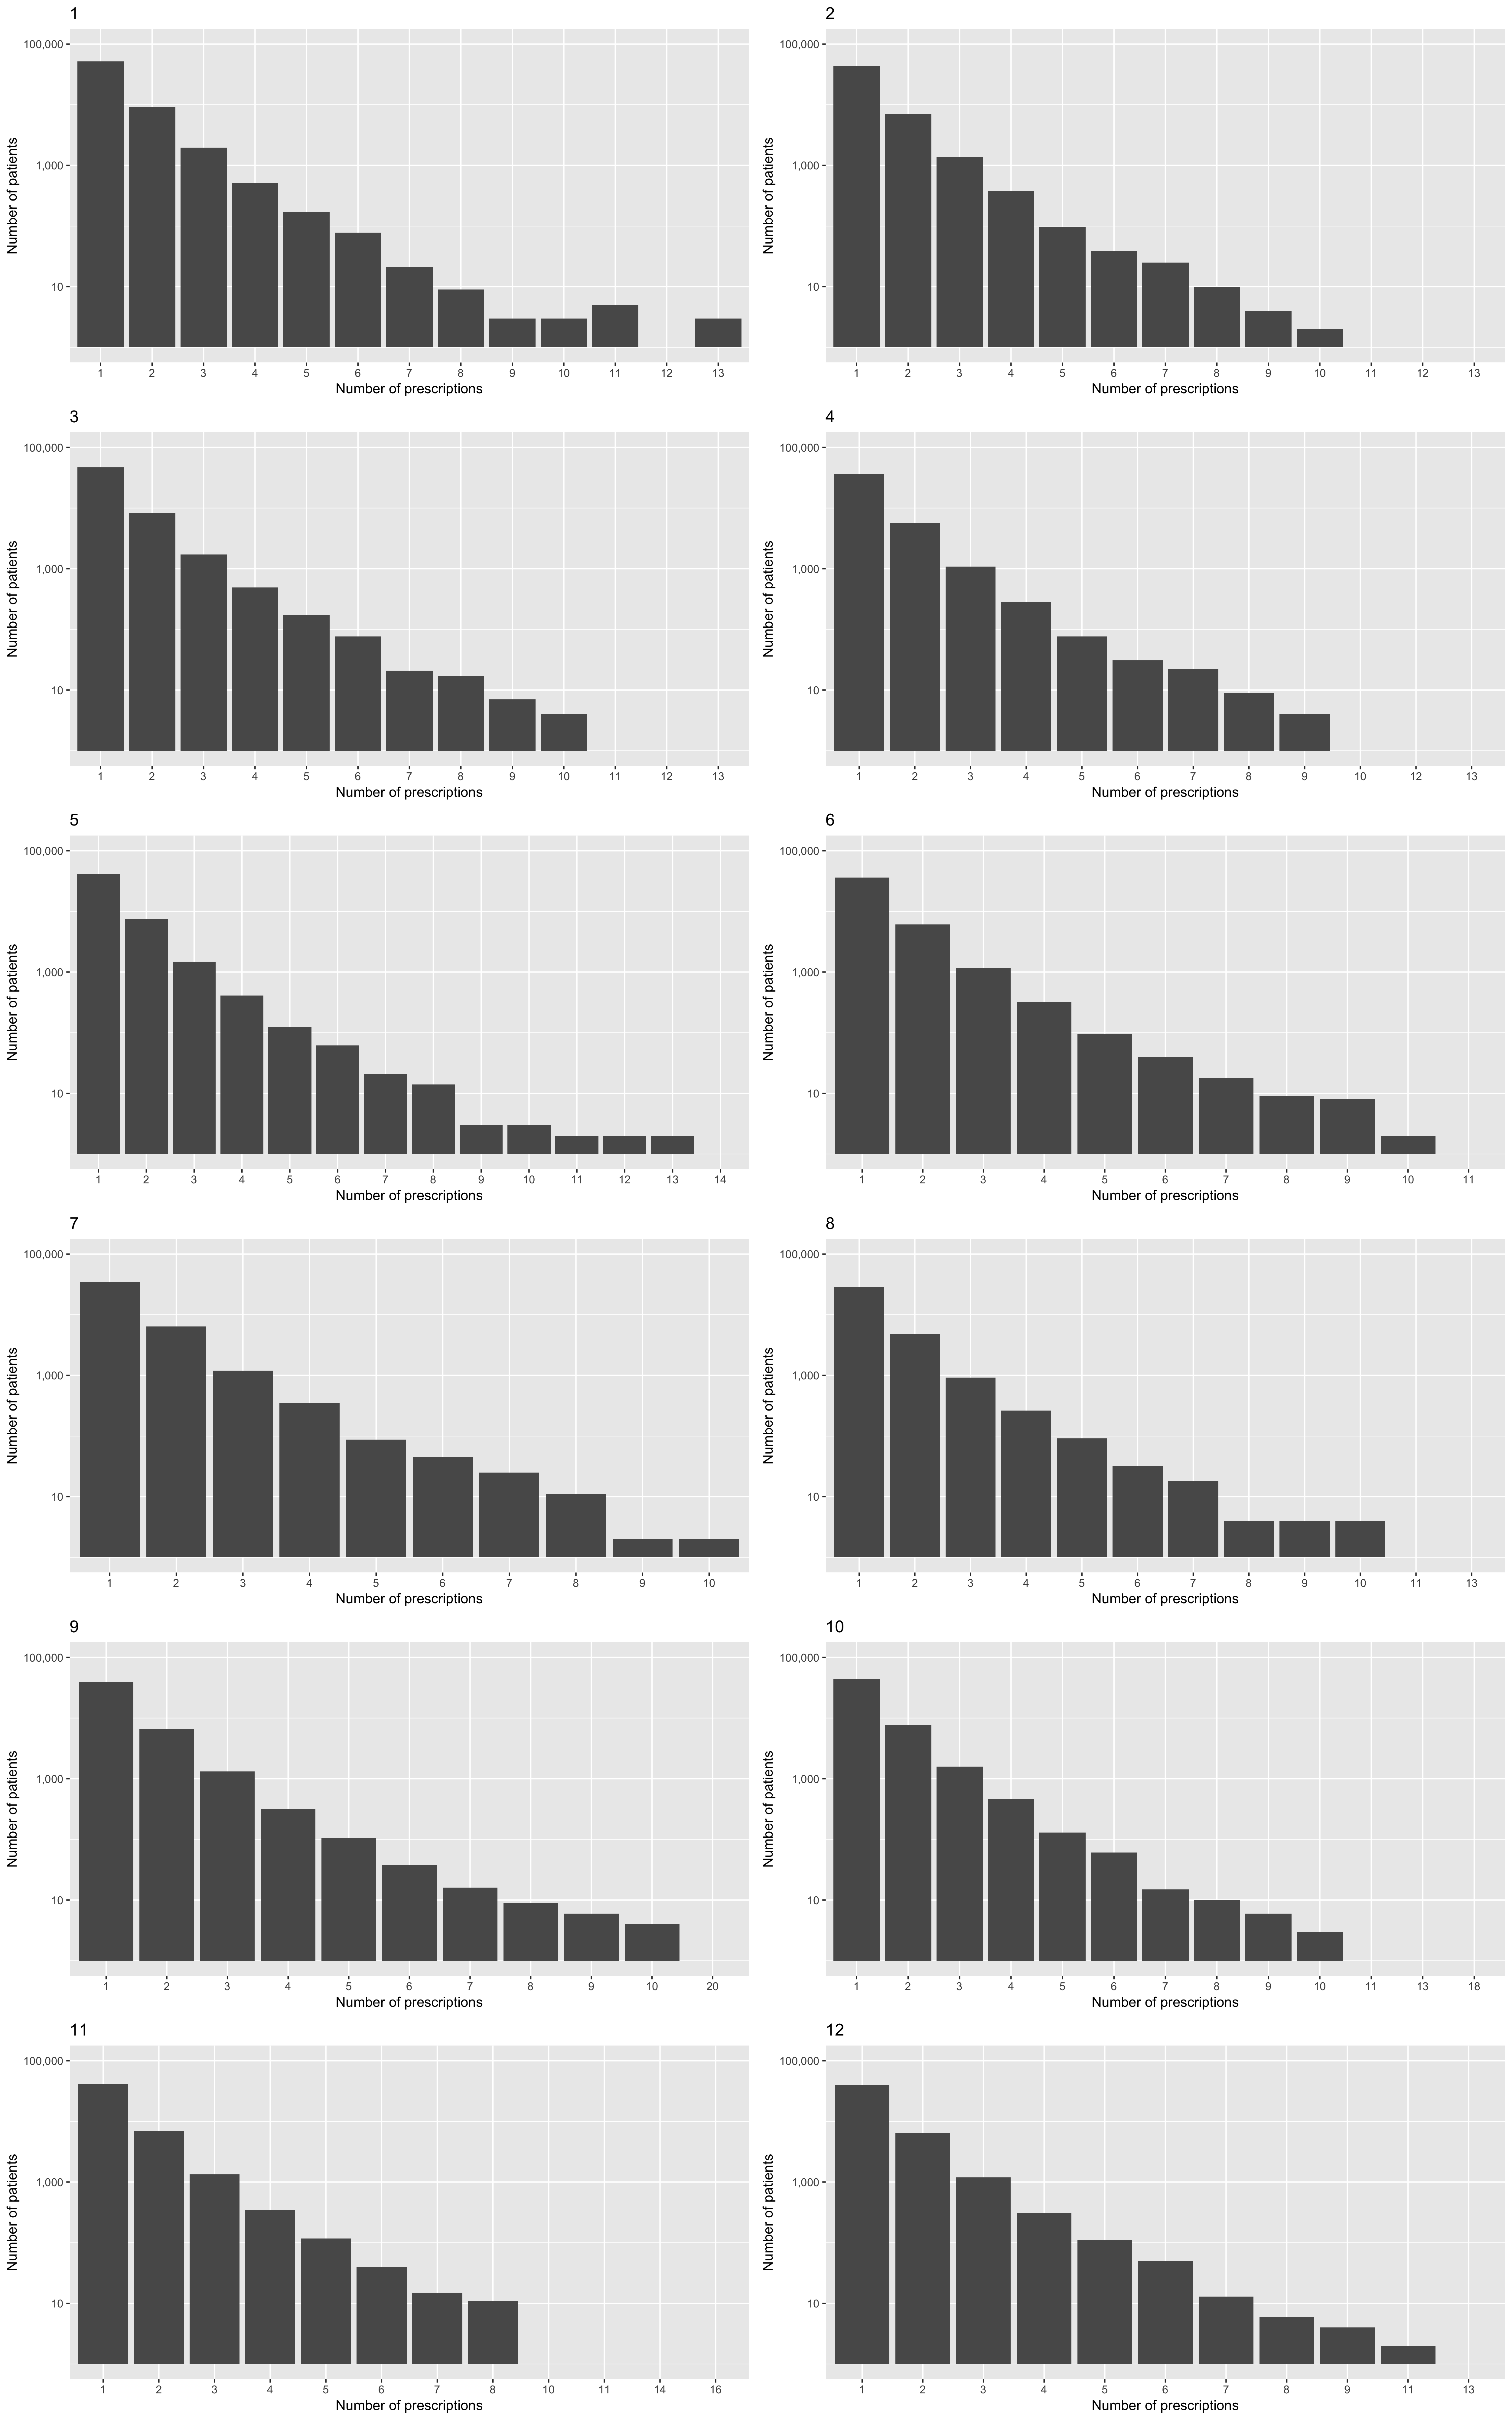
\includegraphics[scale=0.135]{../plots/prescriptions_number-month.png}
\end{figure}

In winter there are more patients having a larger number of prescriptions, while during the summer higher values tend to disappear and even patients with one prescription decrease.

\section{ATC rankings}
For each year and each month, the 3 most common antibiotics are extracted, according to their ATC code. Top 3 changes during the years, hence why there are more than 3 labels in the plots. 
\begin{figure}[h]
	\centering
	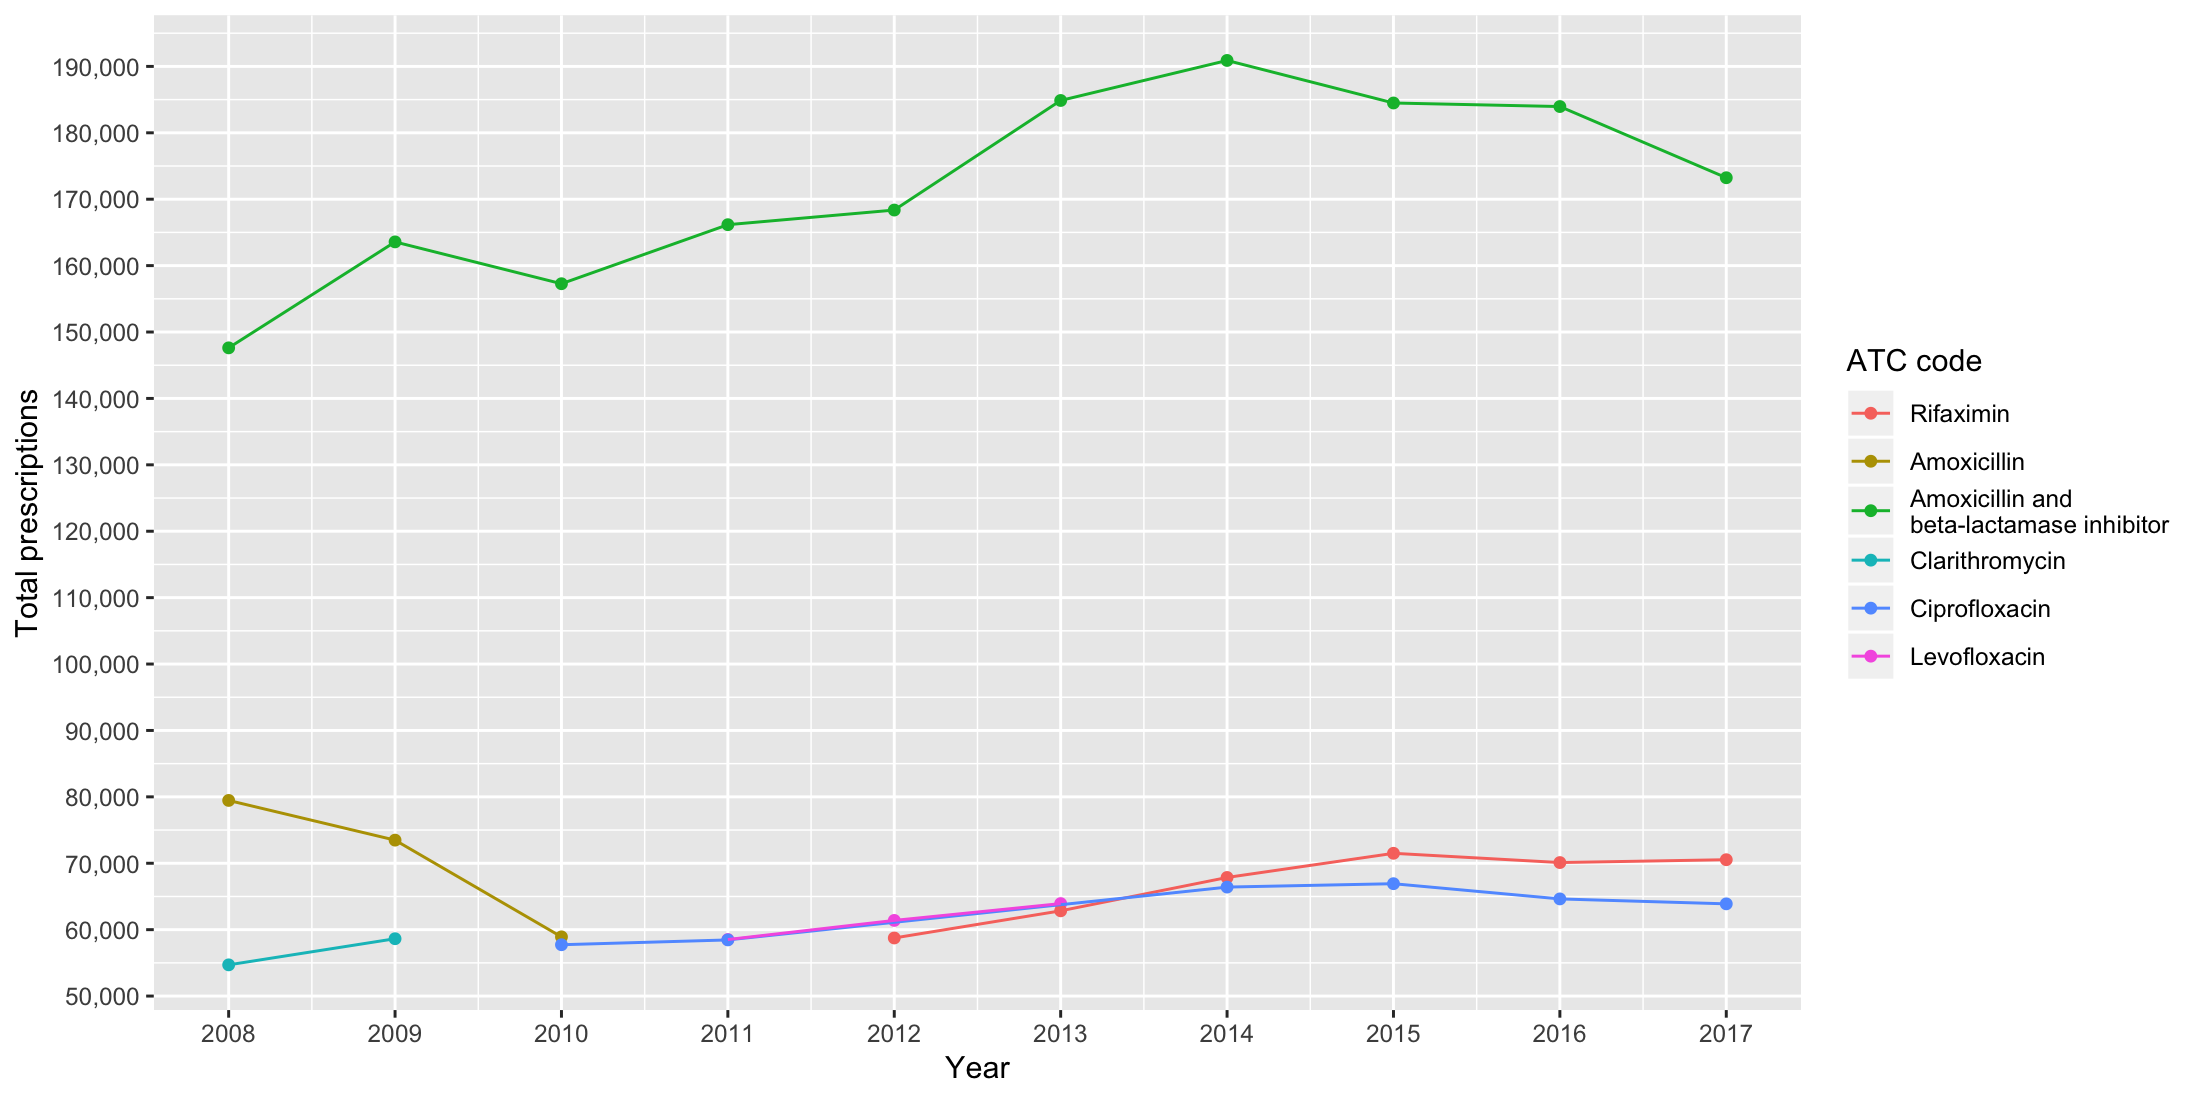
\includegraphics[scale=0.3]{../plots/top_atc-year.png}
\end{figure}

\begin{figure}[h]
	\centering
	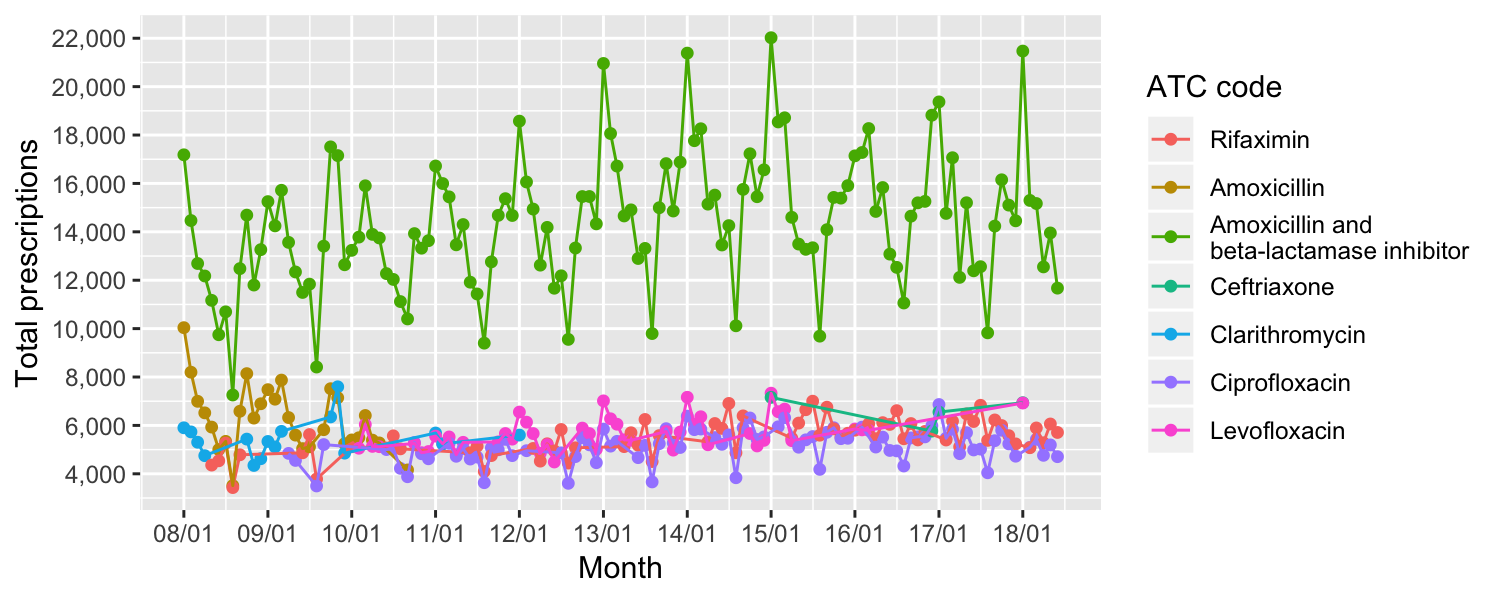
\includegraphics[scale=0.3]{../plots/top_atc-month.png}
\end{figure}

Most ATCs follow a similar pattern: the amount decreases in 2010-2012 to then have a small peak in 2016 and get lower again in 2017, similarly to the global amount of prescriptions.

The most noticeable unusual trend corresponds to amoxicillin and beta-lactose inhibitors (ATC J01CR02), which considerably detaches from the others. Amoxicillin is one of the most popular group of drugs, confirmed by global analytics on the database and USA trends\cite{usa}.

It is evident that the monthly prescriptions follow a seasonal trend: the number of prescription rises during the winter and falls during the summer.

\subsection{Comparison with ICD-9}
Since ICD-9 have some unusual trends, comparing them with antibiotics might provide additional information. The interested area comprehends ICD-9 class A, diseases of the digestive tract whose diagnoses have doubled in the span of 10 years. Antibiotics to treat this subset are:
\begin{itemize}
	\item Nyastatin;
	\item Rifaximin;
	\item Paromomycin.
\end{itemize}

Cross-checking related codes with the antibiotics dataset, rifaximin is indeed one of the most prescribed drugs, while its numbers are still considerably inferior to amoxicillin (the most popular antibiotic). Seasonality is still present, yet less pronounced. 

\begin{figure}[h]
	\centering
	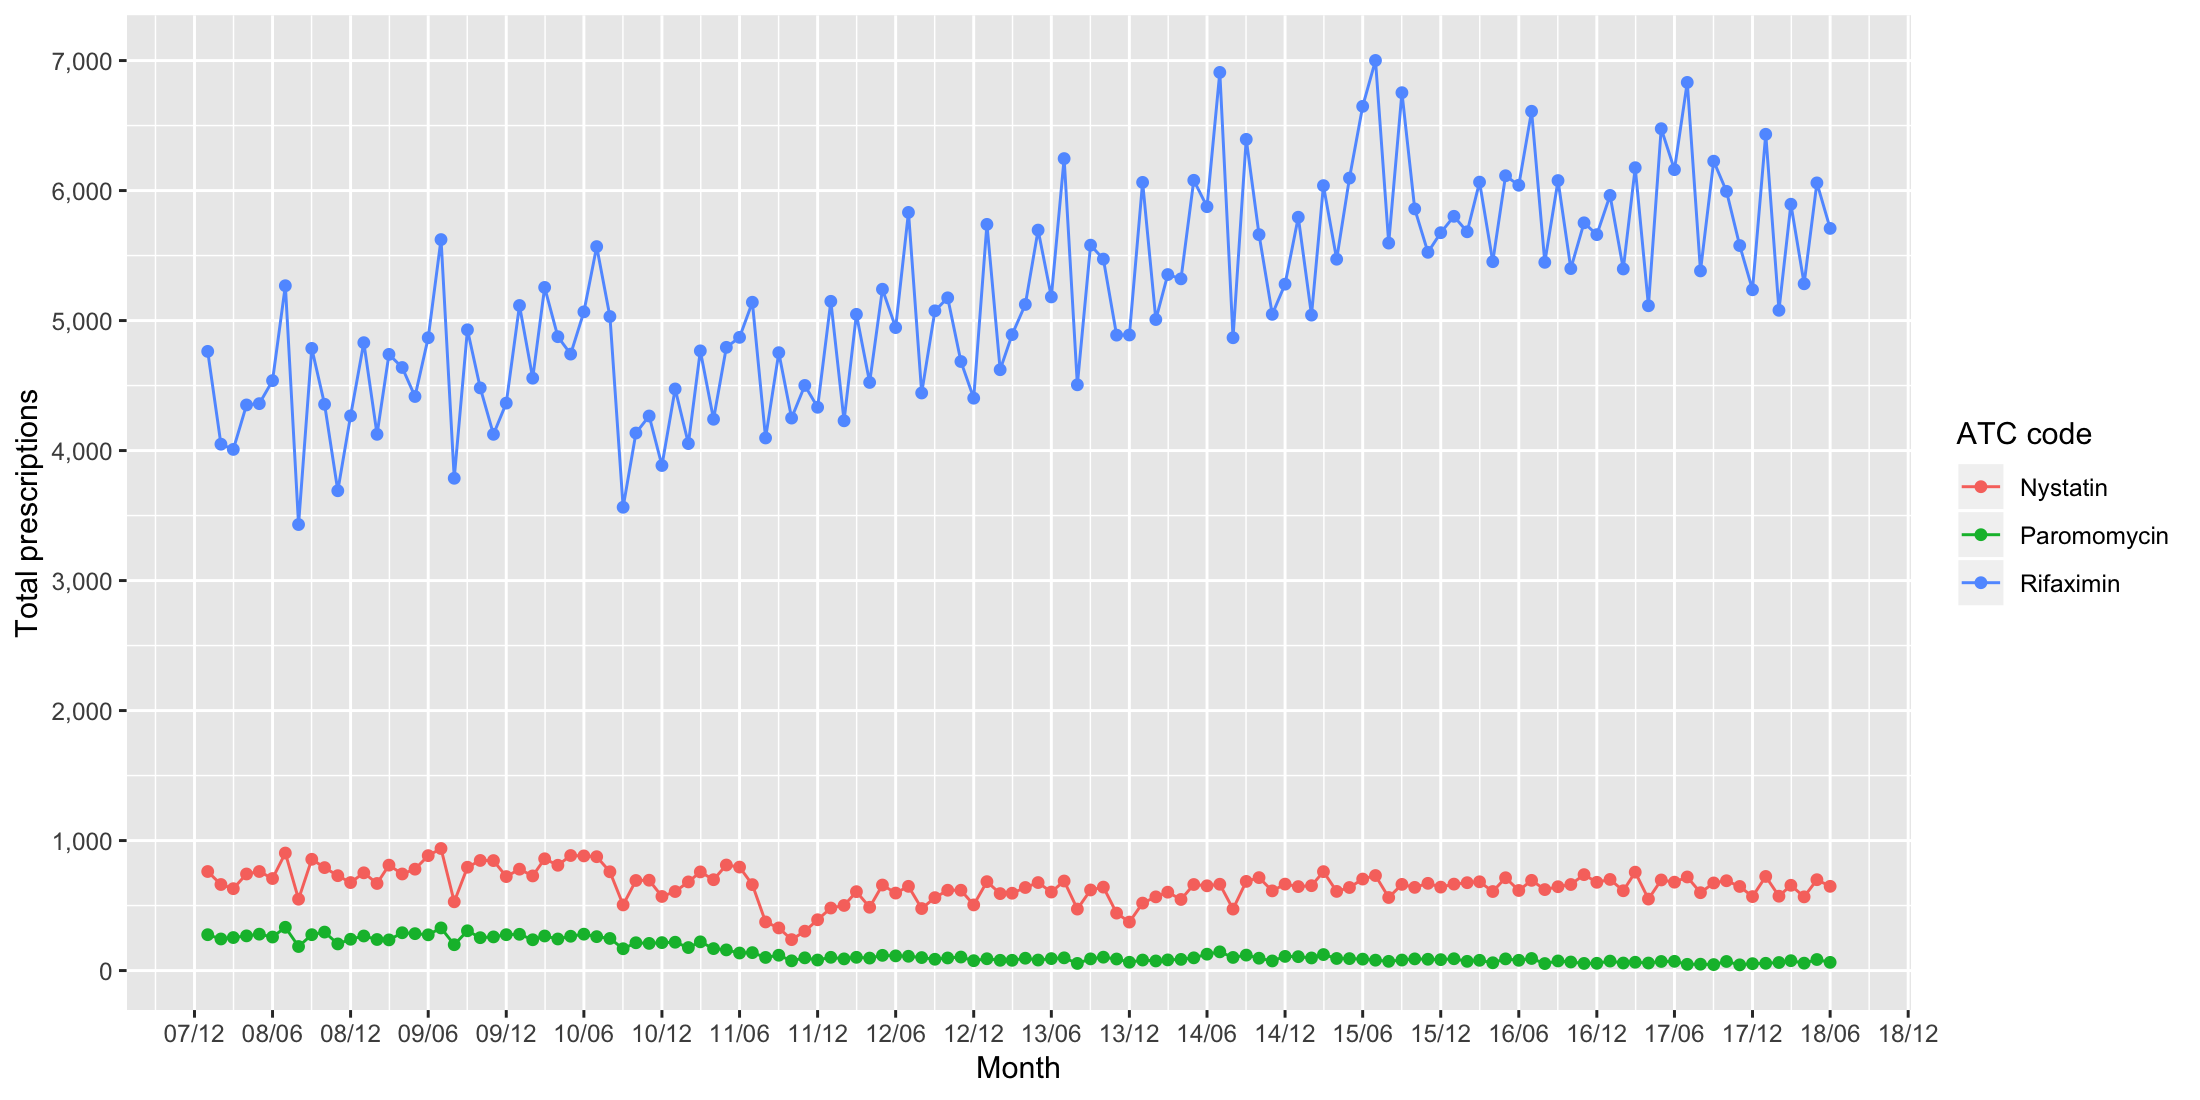
\includegraphics[scale=0.3]{../plots/top_atc_a-month.png}
\end{figure}

\section{AIC rankings}
Prescriptions with AICs don't have a public lookup table, yet drugs can be singularly searched on a public database by AIFA. Analytics have been made on the antibiotics subset of data, using the 5 most prescribed medicines for months and years.

Augmentin is the top ranked prescription, detaching from the others and with a progressive increase starting from 2010: values go up to 100 000 prescriptions in 2017, and January 2017 is the month with the maximum number.

Having a difference of 30 000 between 2010 and 2017 without a correspondent increase of diagnoses shows frequent episodes of antibiotic resistance and overprescribing.

\begin{figure}[h]
	\centering
	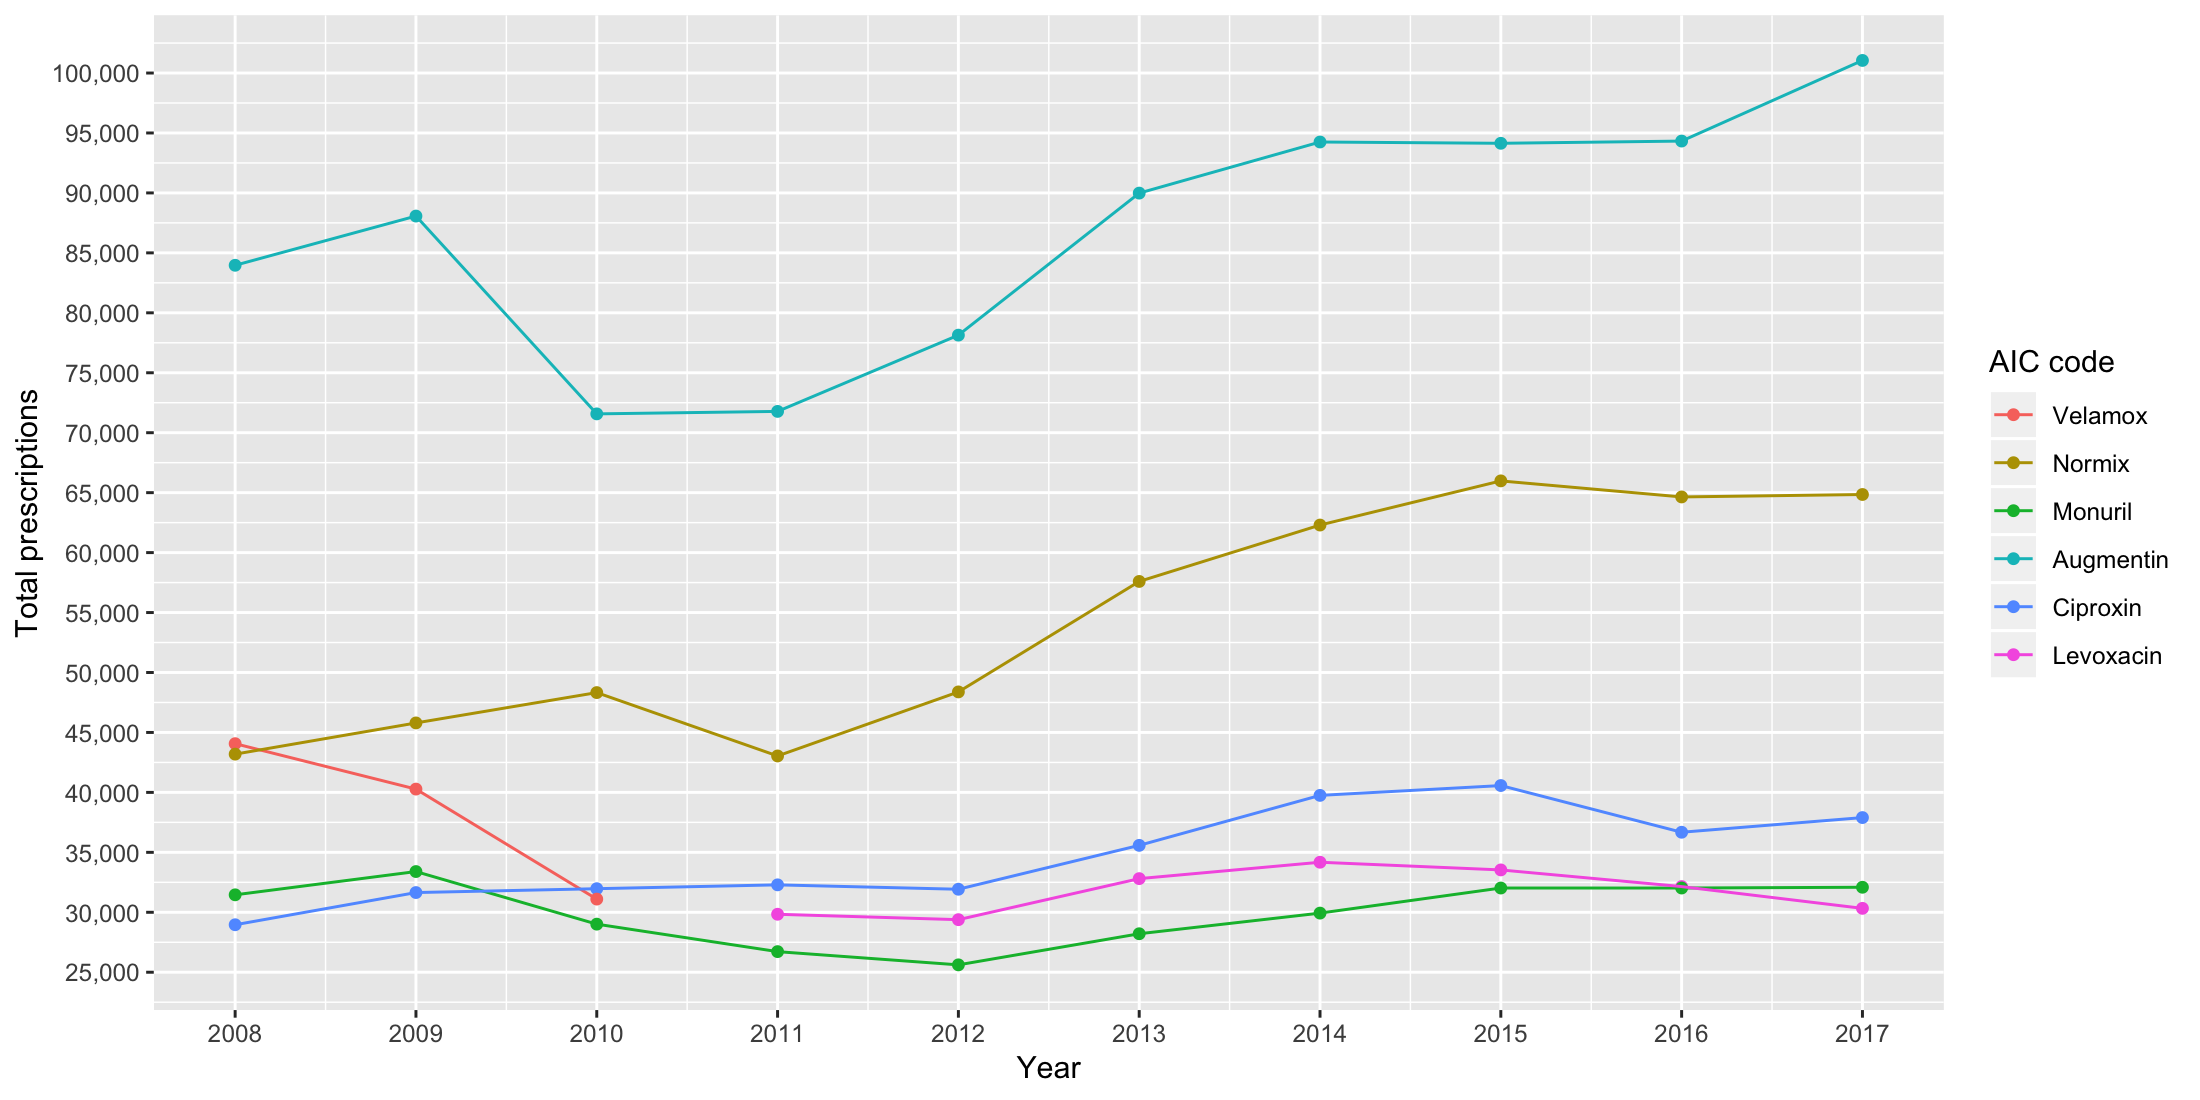
\includegraphics[scale=0.3]{../plots/top_aic-year.png}
\end{figure}

\begin{figure}[h]
	\centering
	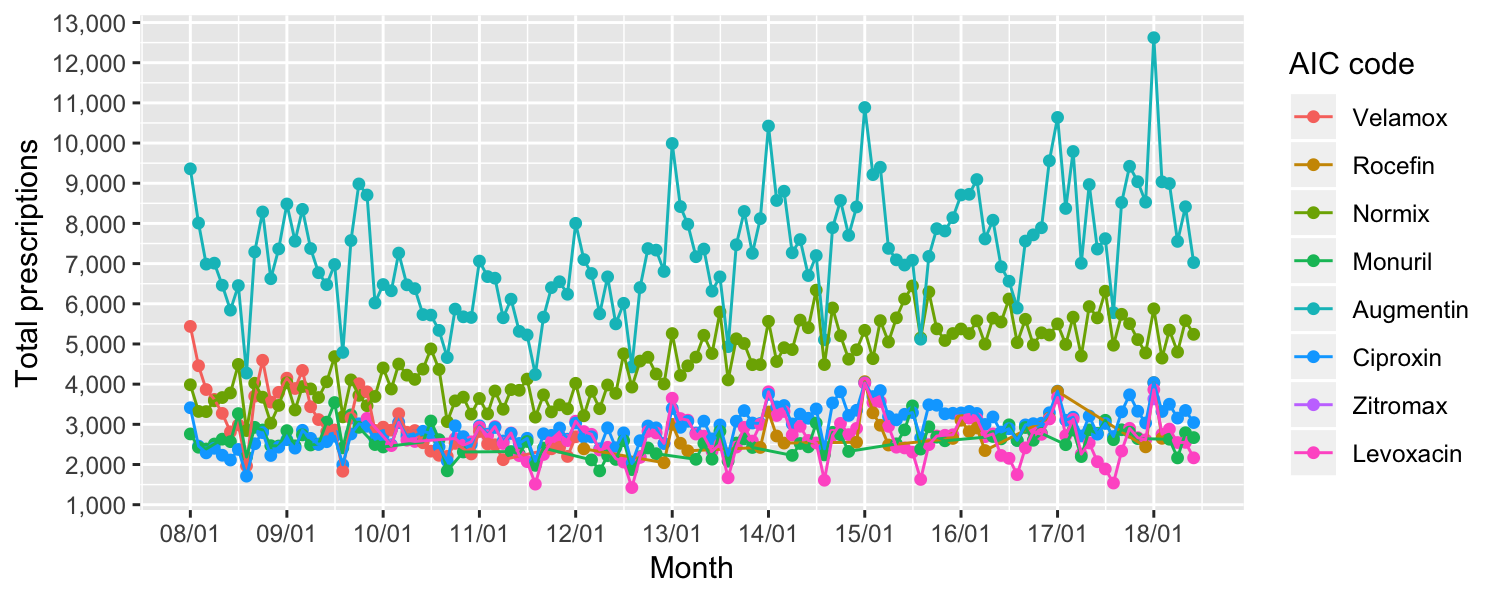
\includegraphics[scale=0.3]{../plots/top_aic-month.png}
\end{figure}

The drug Velamox has an opposite behaviour compared to the others: while most medicines are increasing their number of prescriptions, while Velamox is subject to progressive decrease until disappearance from the most prescribed drugs.

A better understanding between orders of magnitudes could be obtained counting the total prescriptions in 10 years of the most common AICs:

\begin{center}
	\begin{tabular}{|c|c|c|}
		\hline
		Code & Prescriptions & Antibiotic \\
		\hline
		026089019 & 934 942 & Augmentin 875 mg + 125 mg 12 coated tablets \\
		\hline
		025300029 & 586 782 & Normix 200 mg 12 coated tablets\\
		\hline
		026664021 & 373 720 & Ciproxin 500 mg 6 coated tablets \\
		\hline
		033940038 & 264 604 & Levoxacin 500 mg 5 coated tablets \\
		\hline
		025680024 & 229 816 & Monuril 3 g 2 sachets \\
		\hline
		023097102 & 132 787 & Velamox 1 g 12 dispersible tablets \\
		\hline
	\end{tabular}
\end{center}

\subsection{An insight on Velamox}
Velamox, according to AIFA, is an amoxicillin-based drug used for respiratory trait, ear and genital infections. It is sold in different packages, whose the most popular is the 1 g dispersible tablets with 12 tablets.

Since the general trending of most prescribed antibiotics only gave a partial vision of the comparisons between products, a complete chart is extracted using Velamox and three other popular drugs: Augmentin, Normix and Levoxacin. The difference is evident:

\begin{figure}[h]
	\centering
	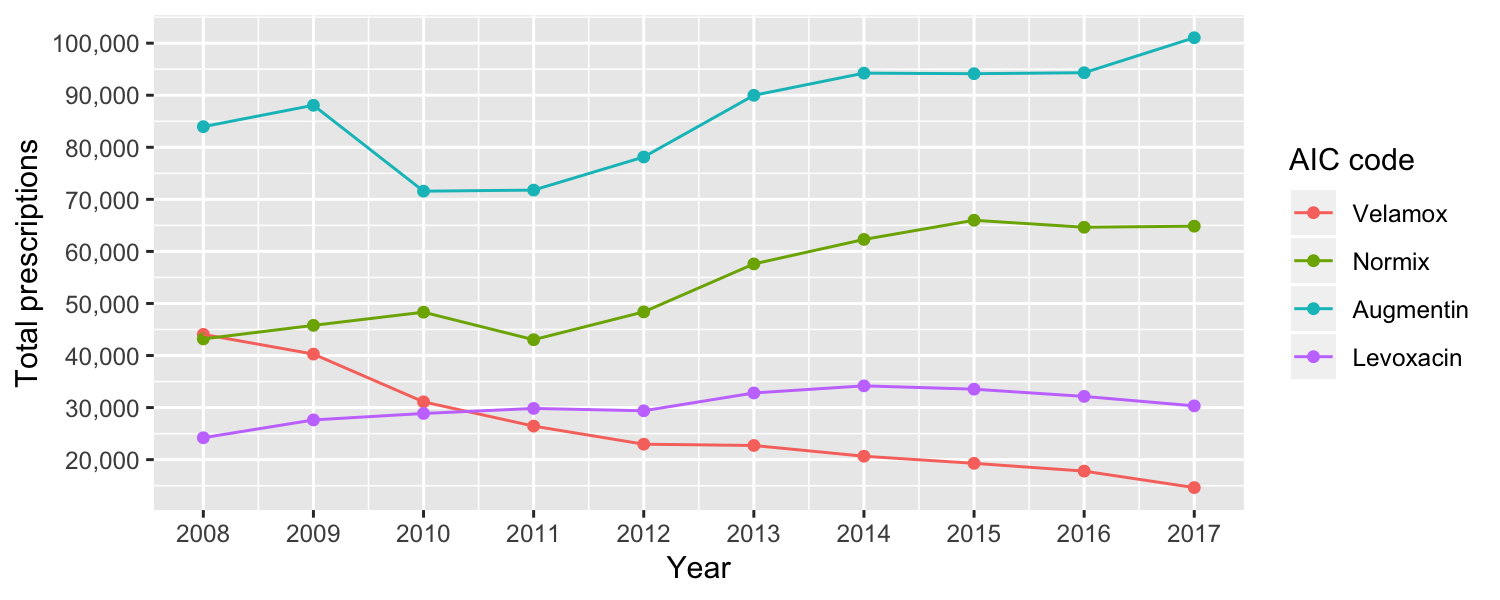
\includegraphics[scale=0.3]{../plots/aic_4-year.png}
\end{figure}

The first hypothesis of such a drastic drop of a product is its switch with another one, changing prescriptive habits of doctors. If that was the case, graphs related to the specific subset of patients would have a correspondent rise of values belonging to another antibiotic.

Velamox in 2008, the year of maximum amount of prescriptions, has been given to approximately 32 000 patients. Extracting only the top 3 antibiotic prescriptions of those, in the last 10 years, along with Velamox, shows no substitution by another drug.

The fall starts in 2009, having a drop of 30 000 units, and gradually continues until 2017 with only 3 037 prescriptions:

\begin{figure}[h]
	\centering
	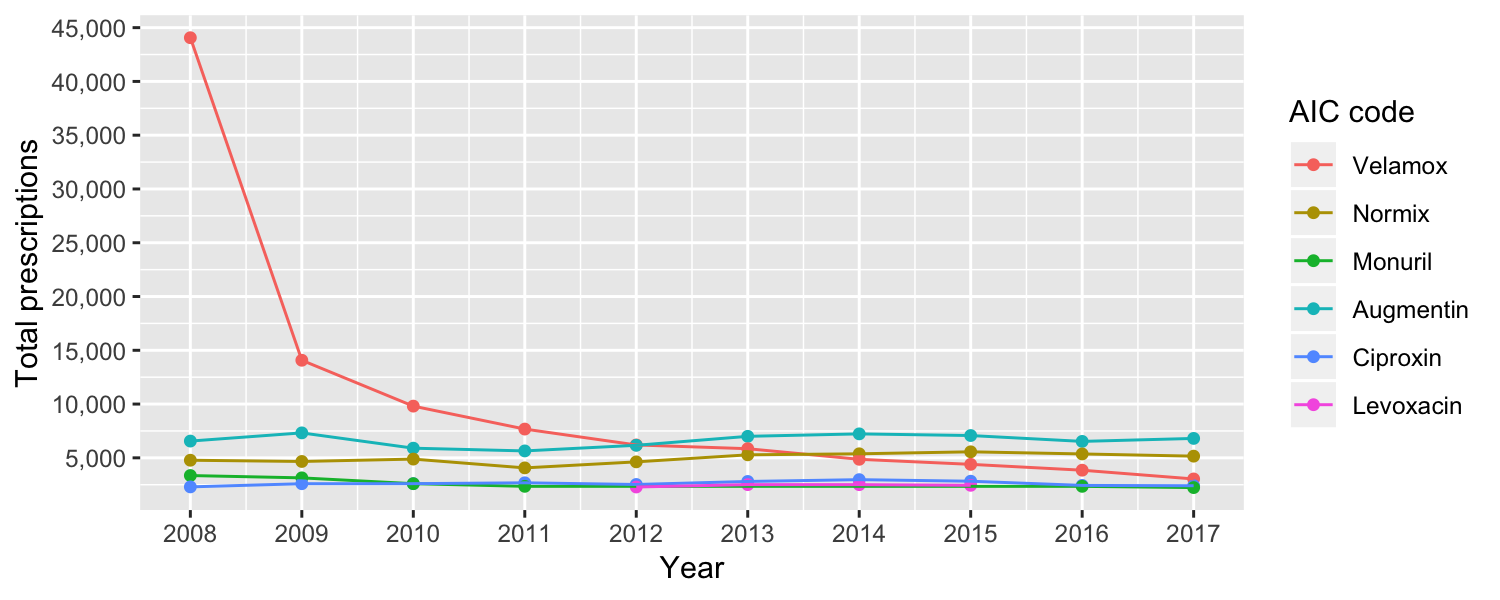
\includegraphics[scale=0.3]{../plots/top_aic_subset-year.png}
\end{figure}

ATC trends related to Velamox's AIC show usual patterns: since the same ATC is linked with more products, the curve is still leaning upwards, yet there is an offset equal to the decrease in Velamox.

Since analysis on a subset of patients gives little insight, a wider time range can give additional information on a complete picture of global trends. 

Further knowledge is obtained counting the total number of Velamox prescriptions among all patients from 2000 to 2017:

\begin{figure}[h]
	\centering
	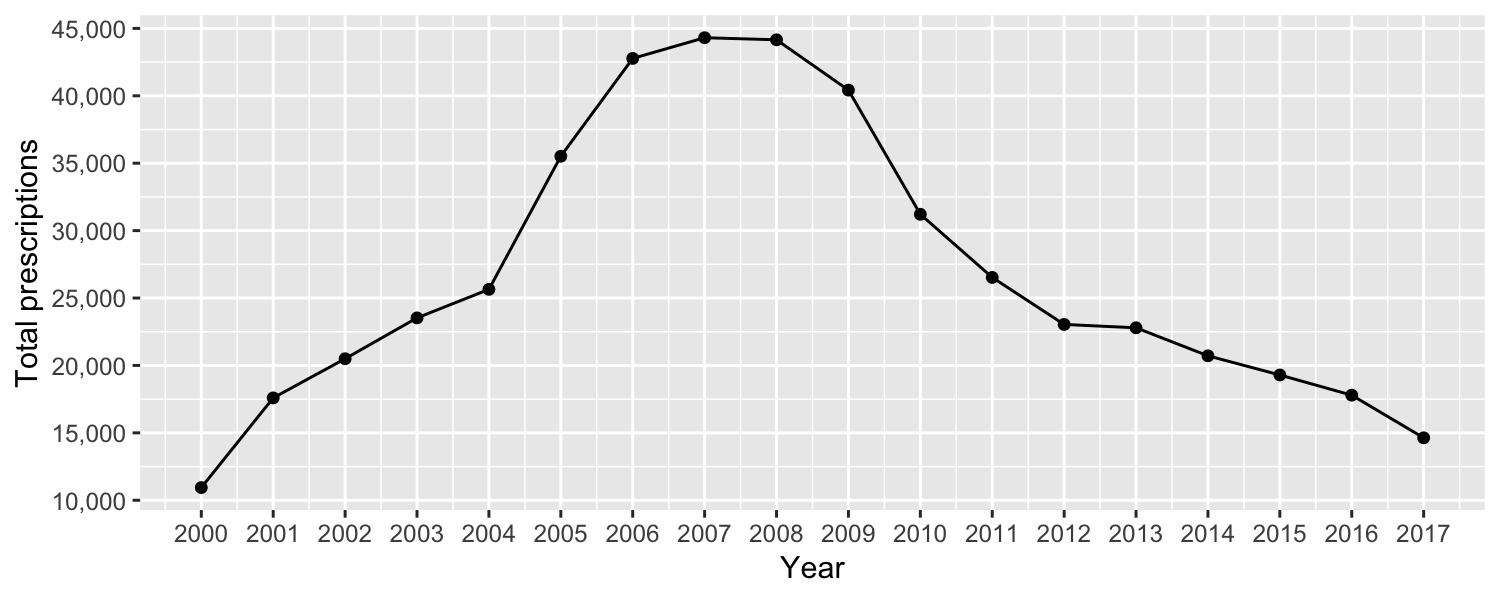
\includegraphics[scale=0.3]{../plots/velamox-year.png}
\end{figure}

Velamox has acquired popularity from 2005 to 2010, when antibiotic resistance still hadn't been recognised as a problem and before the advent of generic drugs, yet this does not provide an explanation for the decrease.

Additional analysis is made on the subset of 32 000 patients:
\begin{itemize}
	\item 1 500 are dead;
	\item 8 000 have changed GP;
	\item 18 000 are females;
	\item 14 000 are males;
	\item 16 000 are born before 1960.
\end{itemize}

General practitioners assigned to the subset of patients have generally decreased their prescriptions quota, roughly halving it comparing 2008 to 2017.

AIFA has also revoked authorisation for most instances of Velamox packages, only leaving three out of ten. The company which produces the drug, Mediolanum Farmacy, has been acquired by Neopharmed Gentili in 2018.

Summarising, changes in Velamox prescriptions are partially caused by:
\begin{itemize}
	\item Doctors gradually abandoning it after authorisation revoking;
	\item Patients dying or switching doctor;
	\item Substitutions with other drugs, none of whose is prescribed enough to have a significant trend, such as generics;
	\item Different advertisement campaigns after the company acquisition.
\end{itemize}

\subsection{An insight on Augmentin}
After analysing a drug with an unusual decrease, the focus can shift to the opposite side, considering the one with a noticeable increase.

Augmentin is the most prescribed antibiotic, with an almost constant positive trend:

\begin{figure}[h]
	\centering
	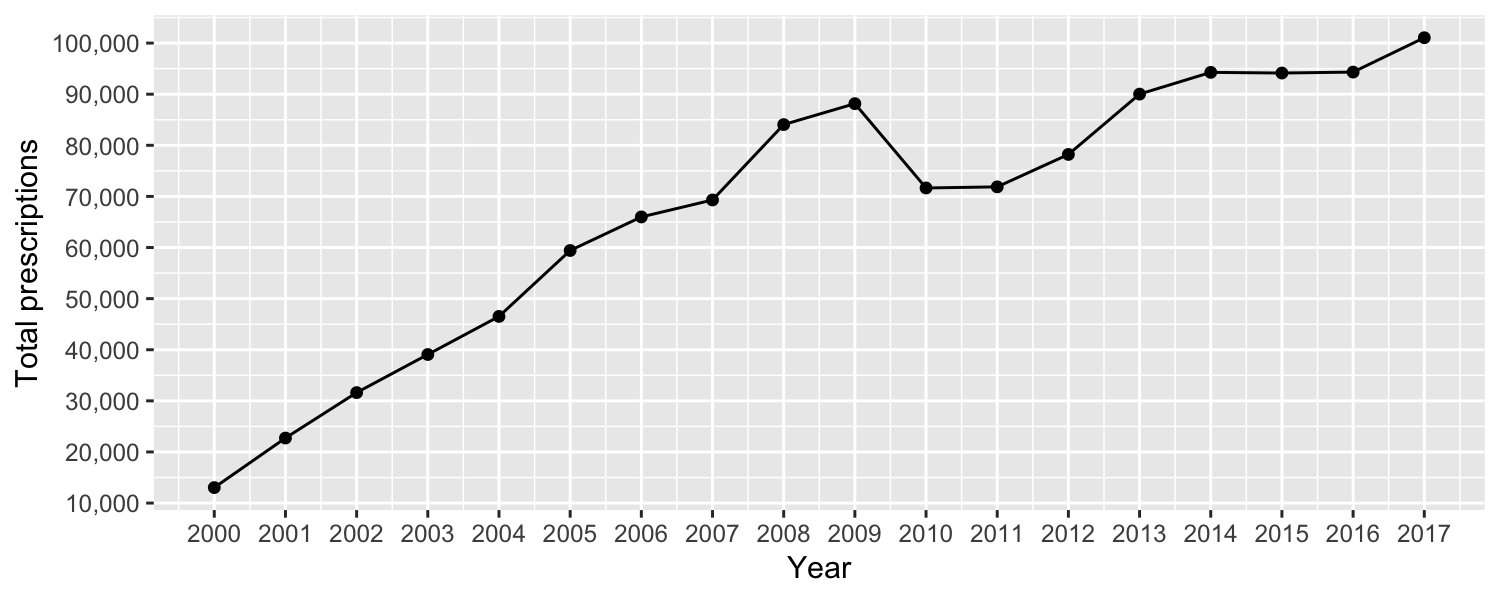
\includegraphics[scale=0.3]{../plots/augmentin-year.png}
\end{figure}

2010 and 2011 have lower values, possibly explained by the Italian economic crisis or the diffusion of generic drugs. Starting from 2013 numbers continue to rise, reaching their highest peak in 2017.

Most Augmentin consumers are adults in the range of 45-64 years of age, following global trends previously obtained.

\begin{figure}[h]
	\centering
	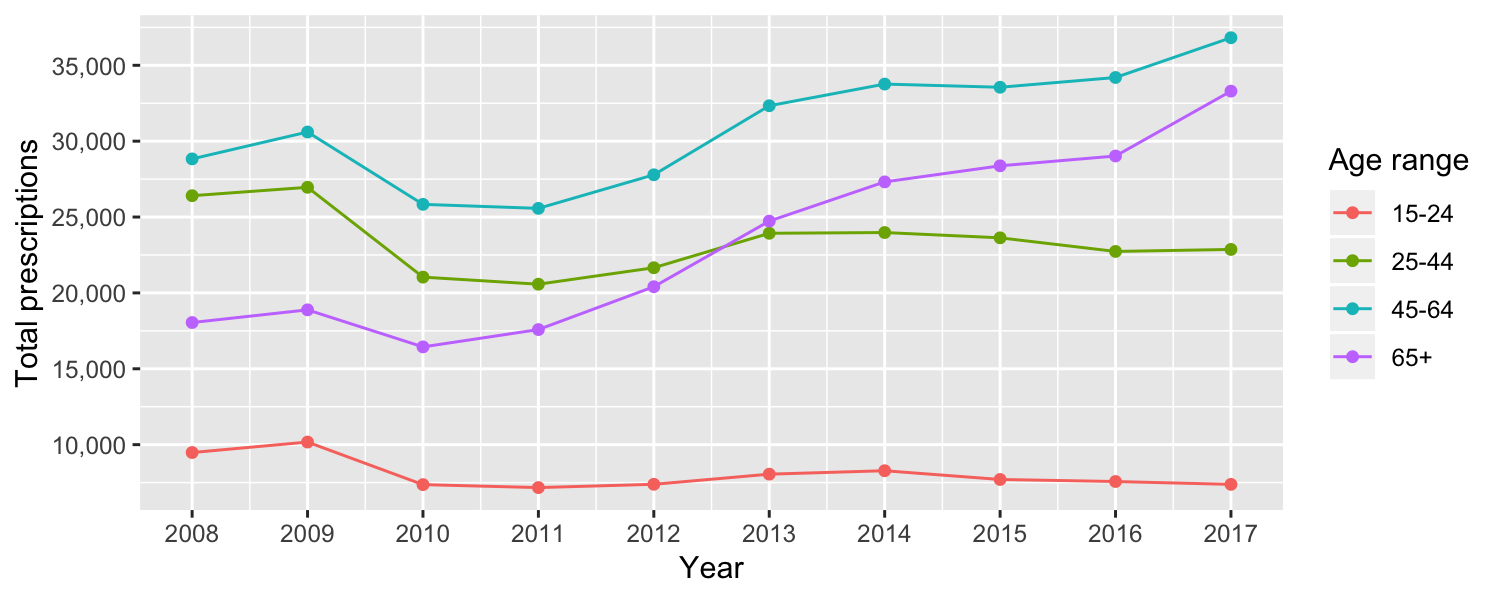
\includegraphics[scale=0.3]{../plots/augmentin_age-year.png}
\end{figure}

\subsection{According to geographical area}
There is information loss on geographical area of patients, therefore it is necessary to extract a further subset of antibiotic prescriptions, applying a level of cleansing.

Patients with complete and correct province of residence fields are selected, obtaining:
\begin{itemize}
	\item 590 472 patients, 74,34\%;
	\item 7 458 312 prescriptions, 88,94\%.
\end{itemize}

Campania has five provinces: Naples, Avellino, Caserta, Benevento and Salerno. Analytics are expected to show an uniform distribution of prescriptions among those, yet outcomes are skewed towards Naples (significantly bigger) and other cities.

Top 5 municipalities for total prescriptions in 2008-2017:
\begin{center}
	\begin{tabular}{|c|c|c|}
		\hline
		Postcode & Province & Prescriptions \\
		\hline
		063049 & Naples & 2 854 056 \\
		\hline
		063002 & Afragola & 618 519 \\
		\hline
		063024 & Castellammare di Stabia & 497 309 \\
		\hline
		063005 & Arzano & 314 640 \\
		\hline
		063035 & Gragnano & 210.960 \\
		\hline
	\end{tabular}
\end{center}

Prescriptions come from 932 different cities, while there are 550 distinct cities in Campania. This implies a slice of patients having residence in a different place outside the region.

Results might be altered by the non-uniform provenance of doctors and patients (mostly from the Naples area), and other big municipalities have large population although not qualifying as provinces. 

Discrepancies among provinces are also shown by the following plot, identifying trends:
\begin{figure}[h]
	\centering
	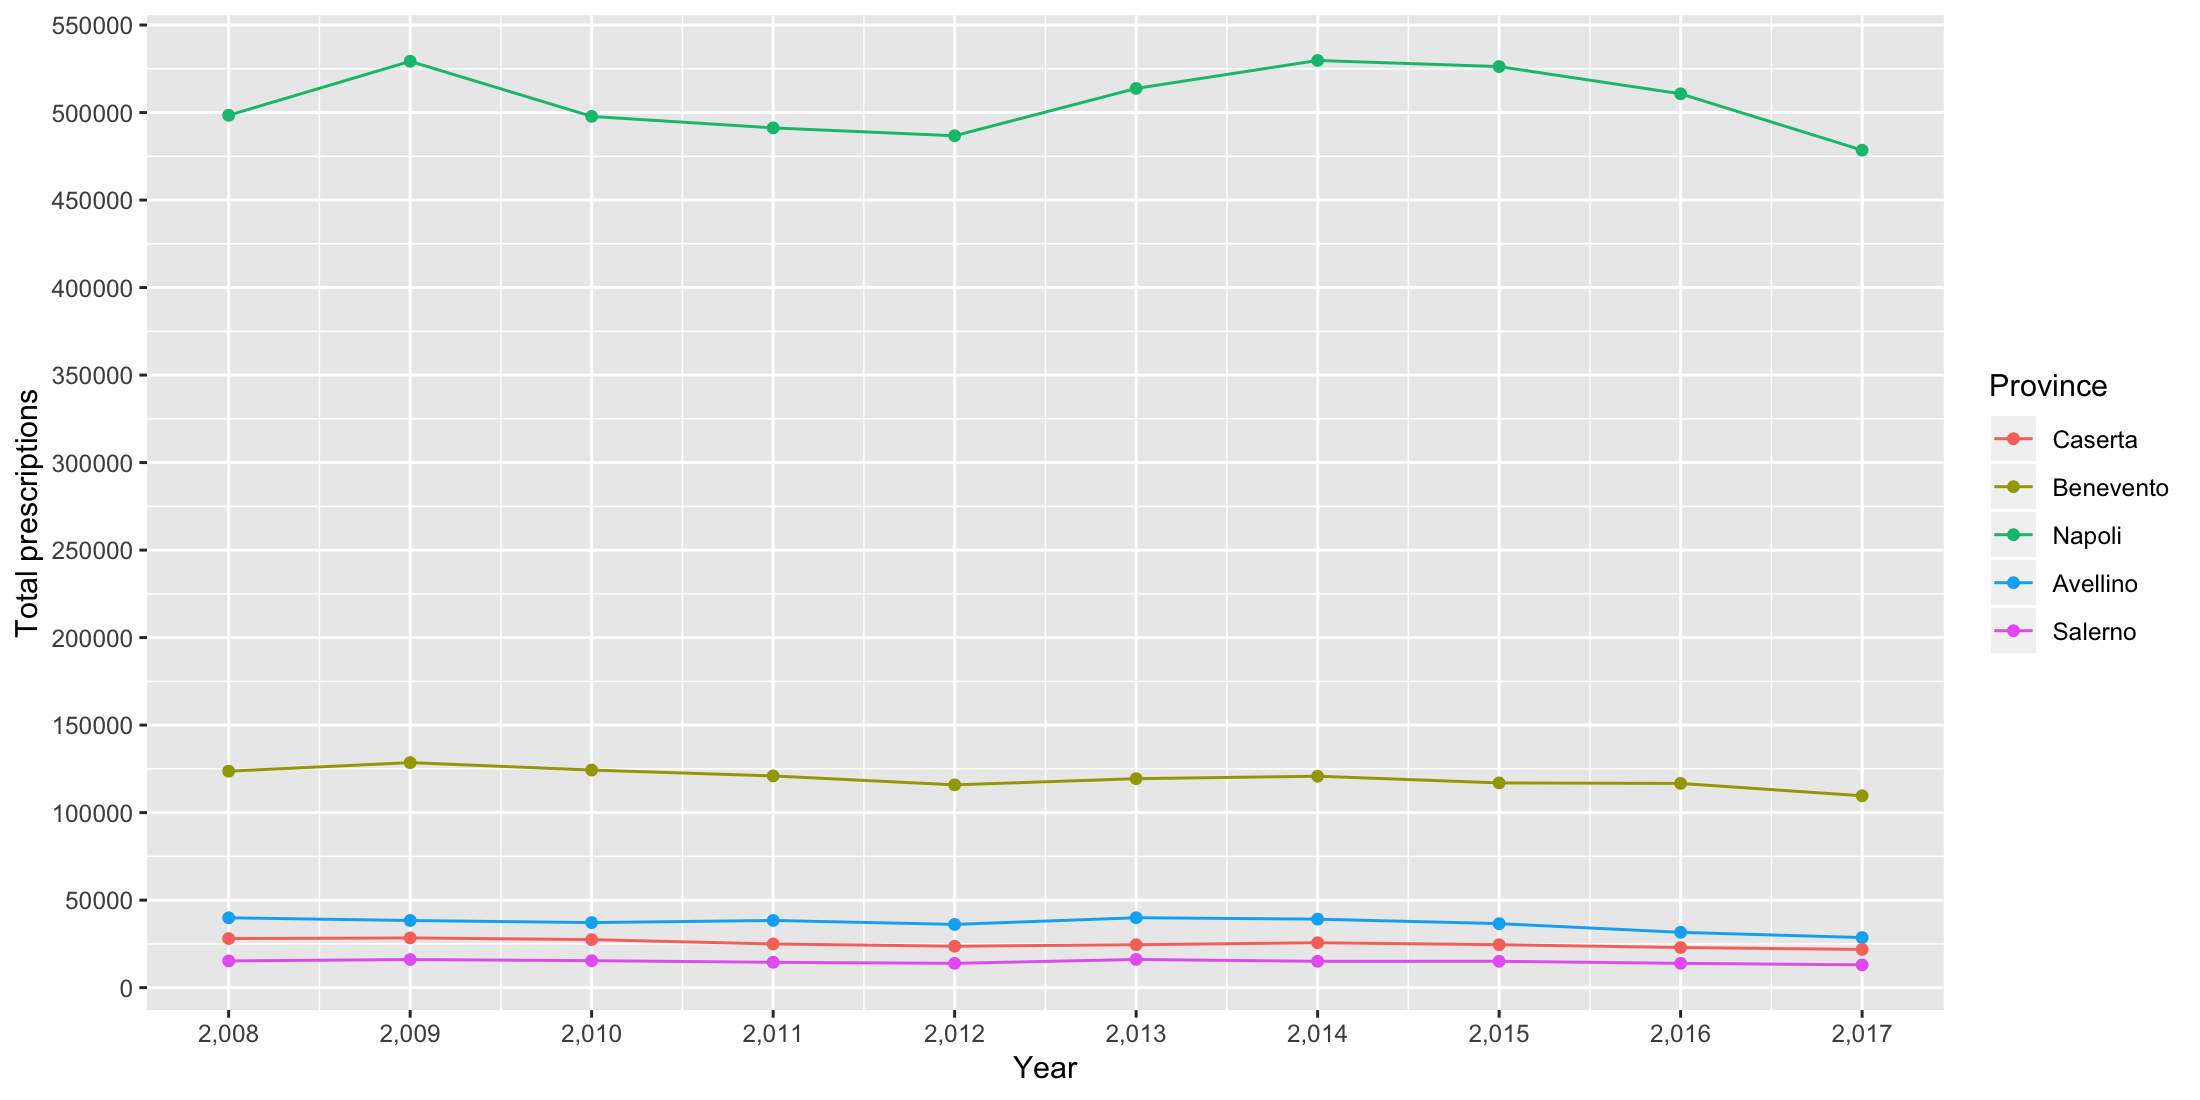
\includegraphics[scale=0.3]{../plots/provinces.png}
\end{figure}

\subsubsection{Pharmacies}
The number of pharmacies divided by province with related population (ISTAT 2018) confirms the gap between Naples and the others: 
\begin{enumerate}
	\item 857 pharmacies in the Naples area, 3 101 002 inhabitants;
	\item 375 pharmacies in the Salerno area, 1 101 763 inhabitants;
	\item 254 pharmacies in the Caserta area, 923 445 inhabitants;
	\item 161 pharmacies in the Avellino area, 421 523 inhabitants;
	\item 107 pharmacies in the Benevento area, 279 127 inhabitants.
\end{enumerate}

\section{ATC and AIC trends}

\subsection{By sex}

\subsection{By age}
Analytics by age are deployed dividing the subset in the 5 official age ranges, however since patients in the youngest group should receive prescriptions by paediatricians and there is no related information in the database, the range 1-14 has to be considered incorrect and therefore removed.

This causes a difference of approximately 150 000 tuples, and the remaining ones are arranged by age of patient counting the amount of prescriptions in 2008-2017:

\begin{center}
	\begin{tabular}{|c|c|c|}
		\hline
		Age range & Prescriptions & Mean\\
		\hline
		15-24 & 643 540 & 5,25 \\
		\hline
		25-44 & 1 776 228 & 7,29 \\
		\hline
		45-64 & 2 674 494 & 10,81 \\
		\hline
		65+ & 3 115 334 & 16,16 \\
		\hline
	\end{tabular}
\end{center}

A patient on average receives 9,8 prescriptions in 10 years, but there are big differences between older and younger people: the number progressively increases.

ATC and AIC popular codes are related, observing that some of the most common ones gets prescribed starting from an early age while others are prevalent between higher ranges.

5 top AICs and ATCs for age, yearly and monthly: % todo fixare i grafici, togliere qualche etichetta

\begin{figure}[h]
	\centering
	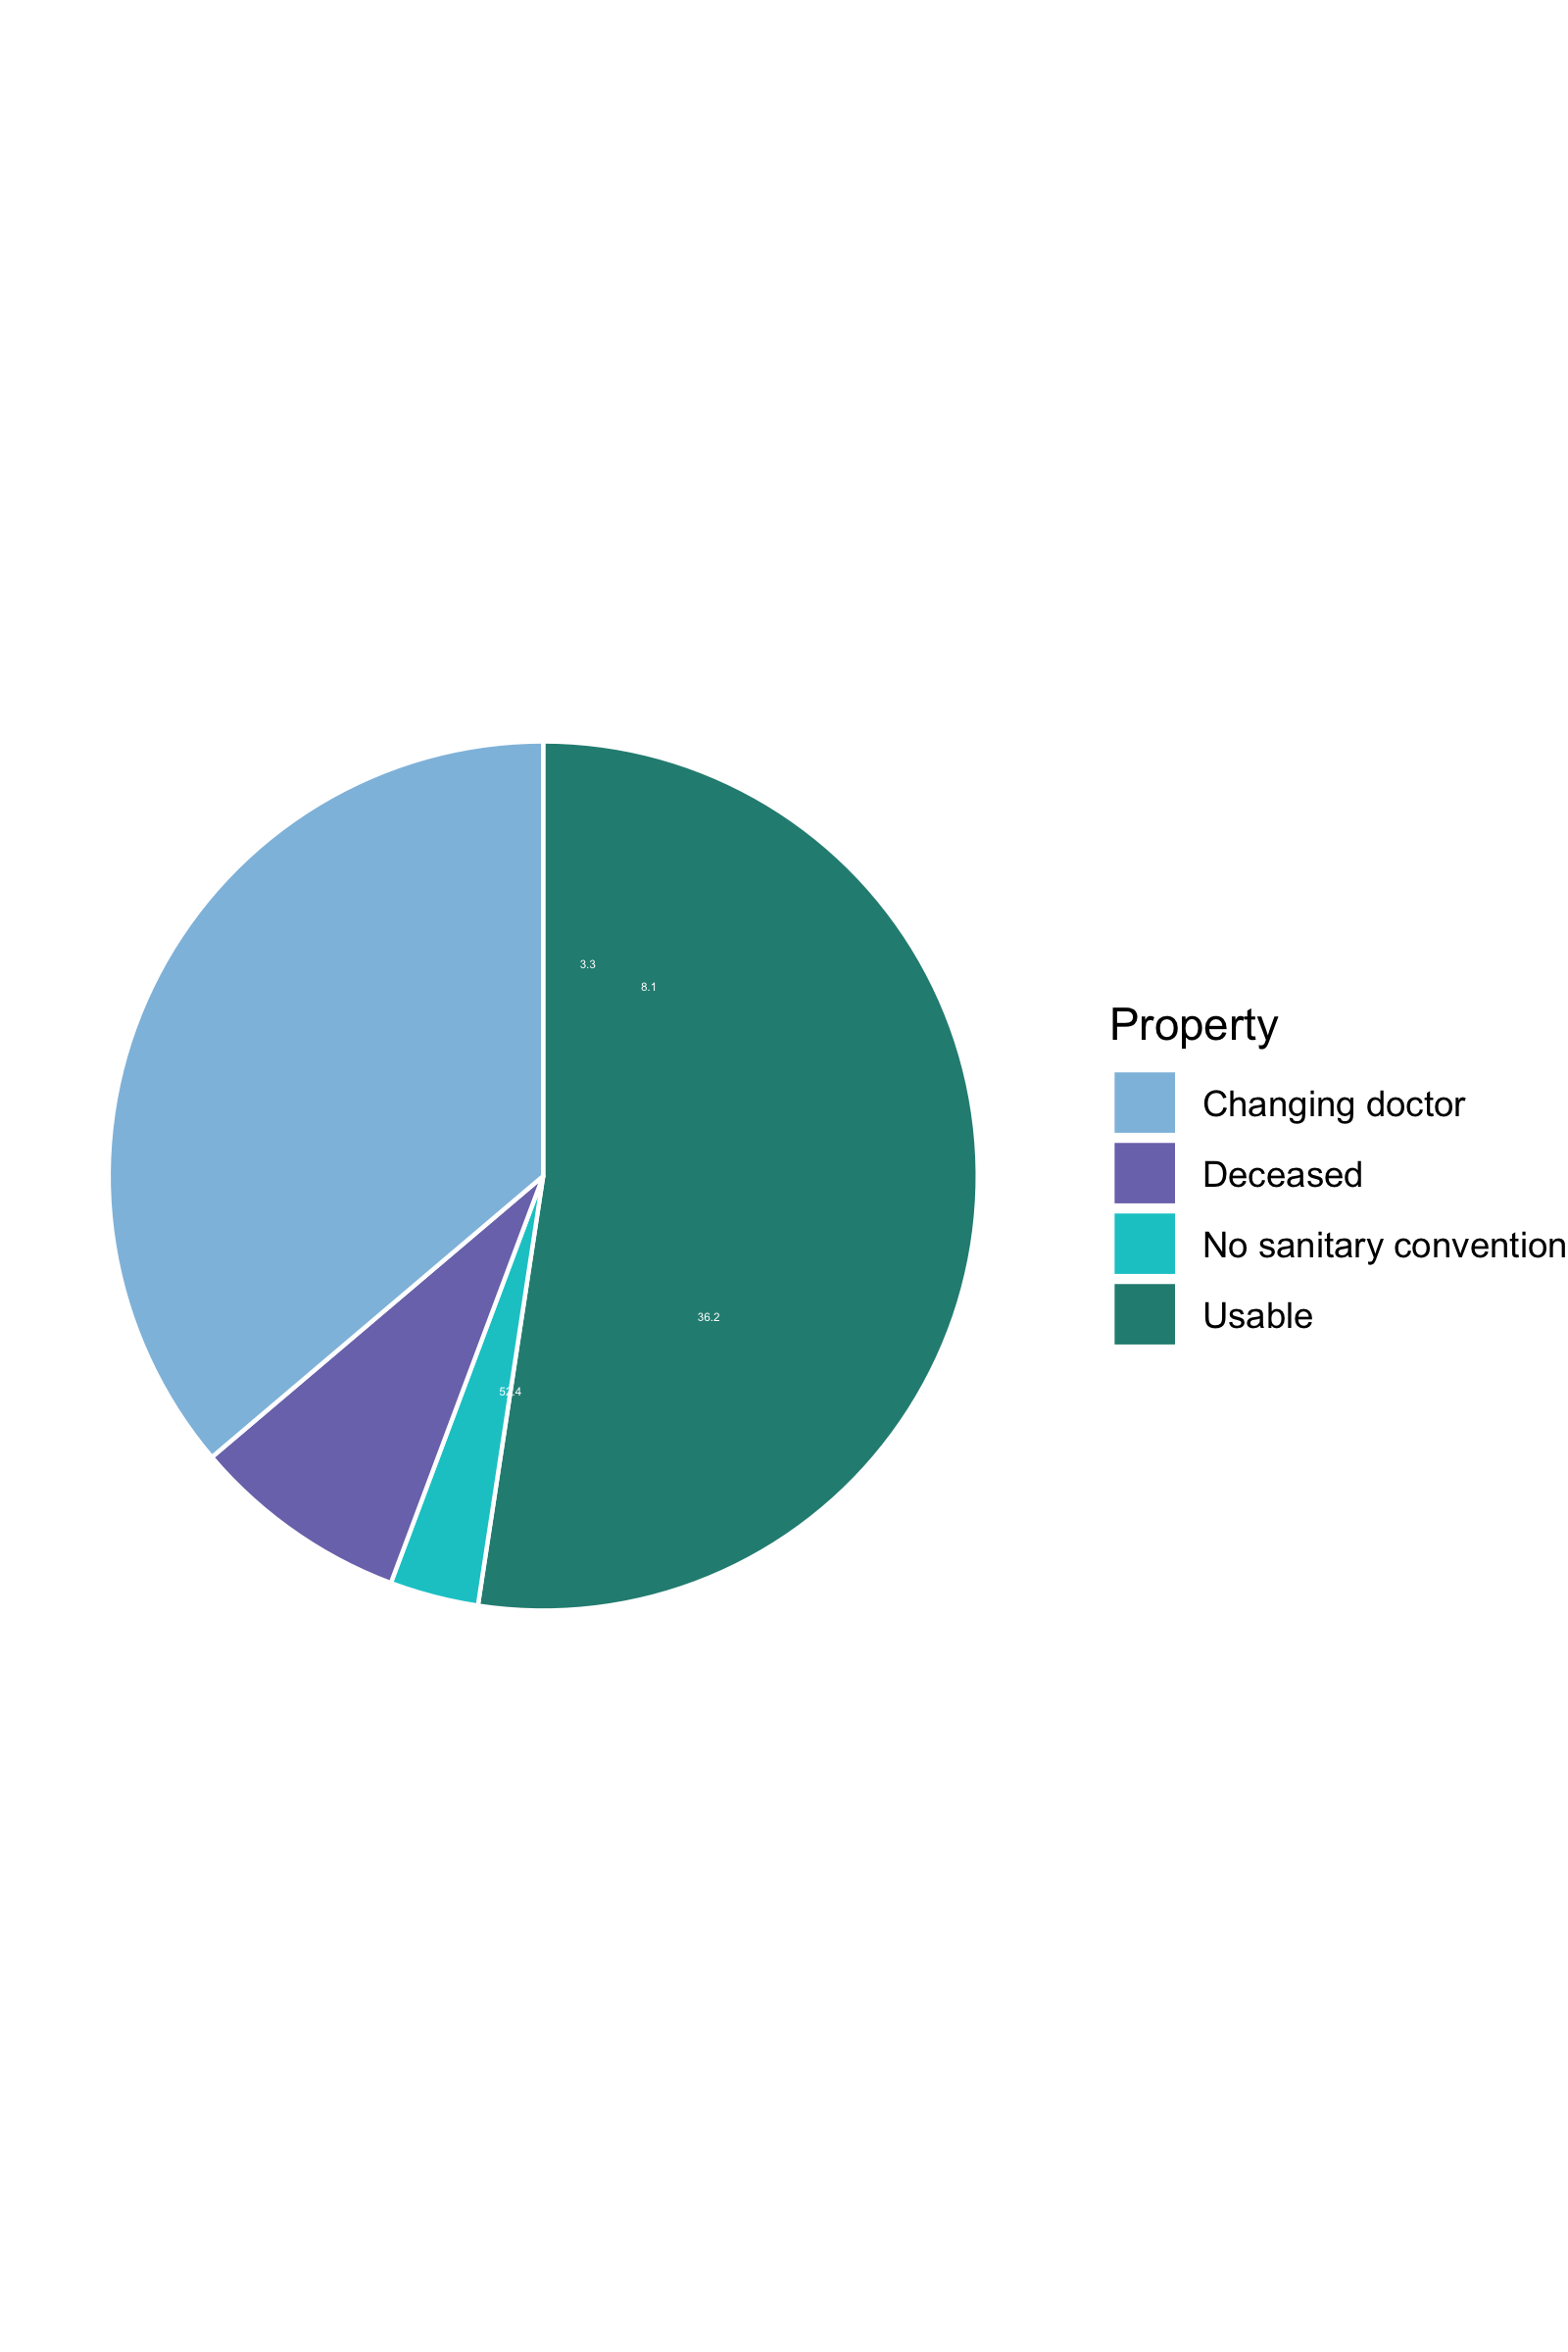
\includegraphics[scale=0.29]{../plots/top_atc_age-year.png}
\end{figure}

\begin{figure}[h]
	\centering
	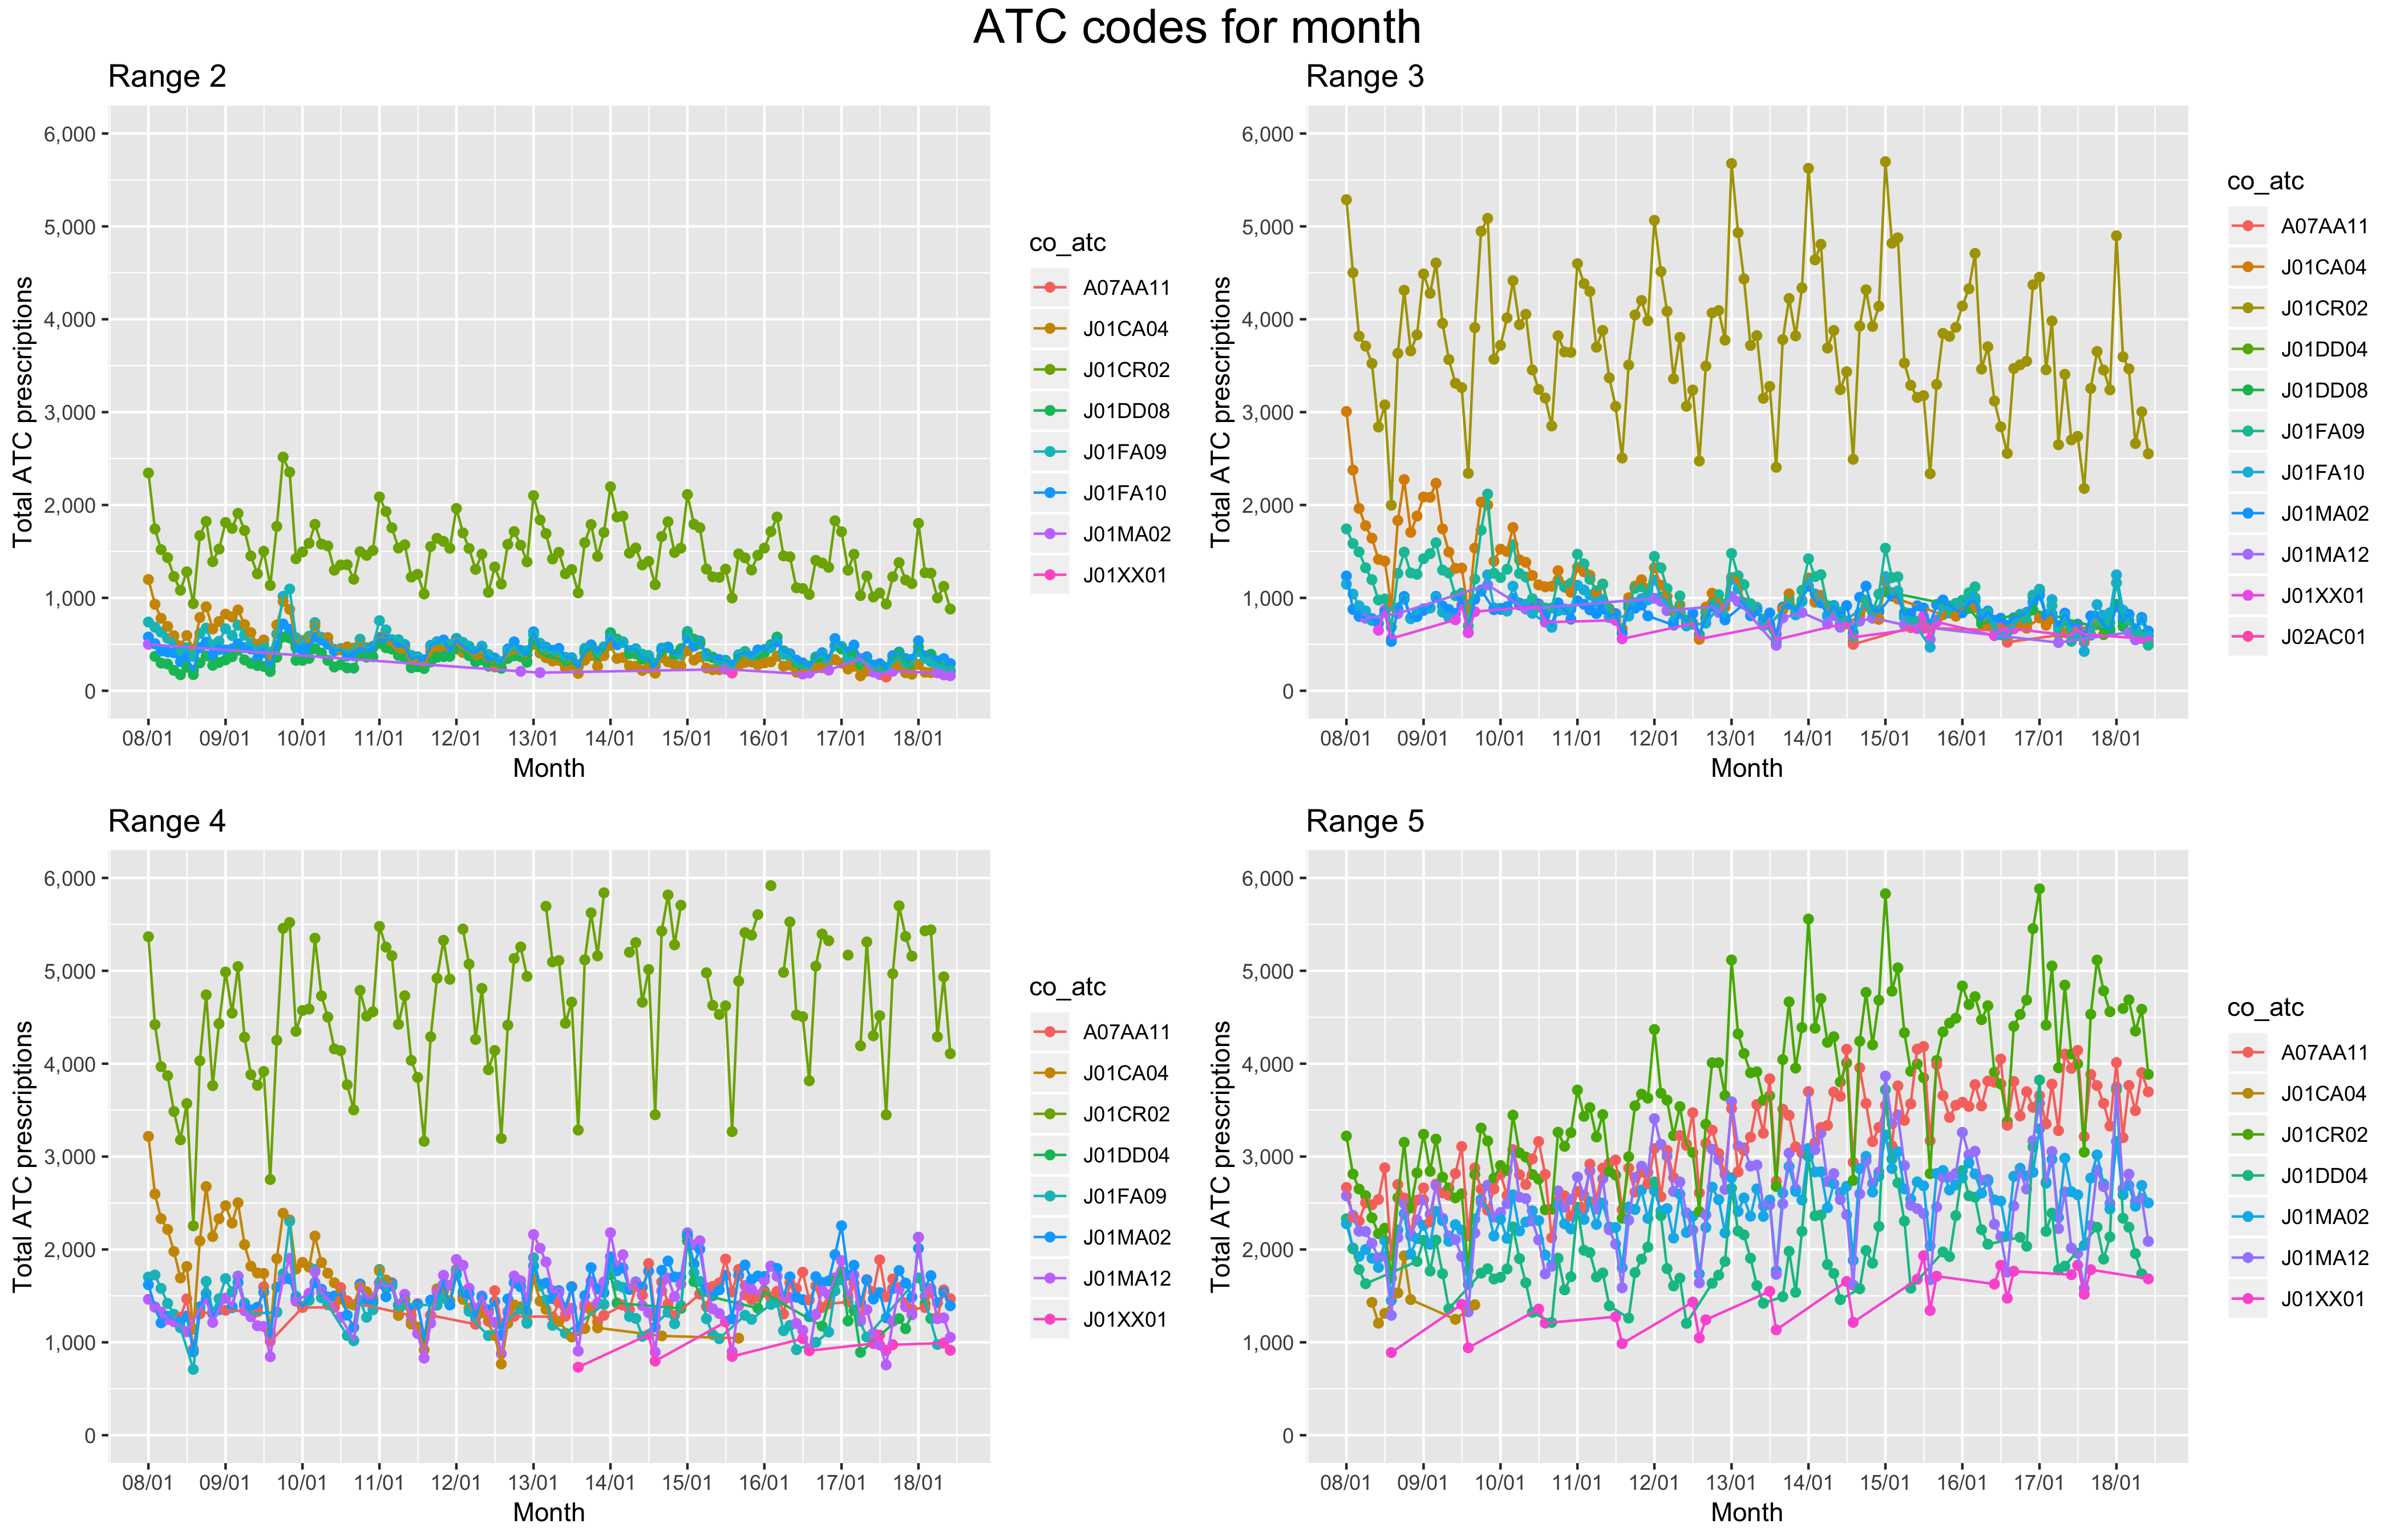
\includegraphics[scale=0.29]{../plots/top_atc_age-month.png}
\end{figure}

\begin{figure}[h]
	\centering
	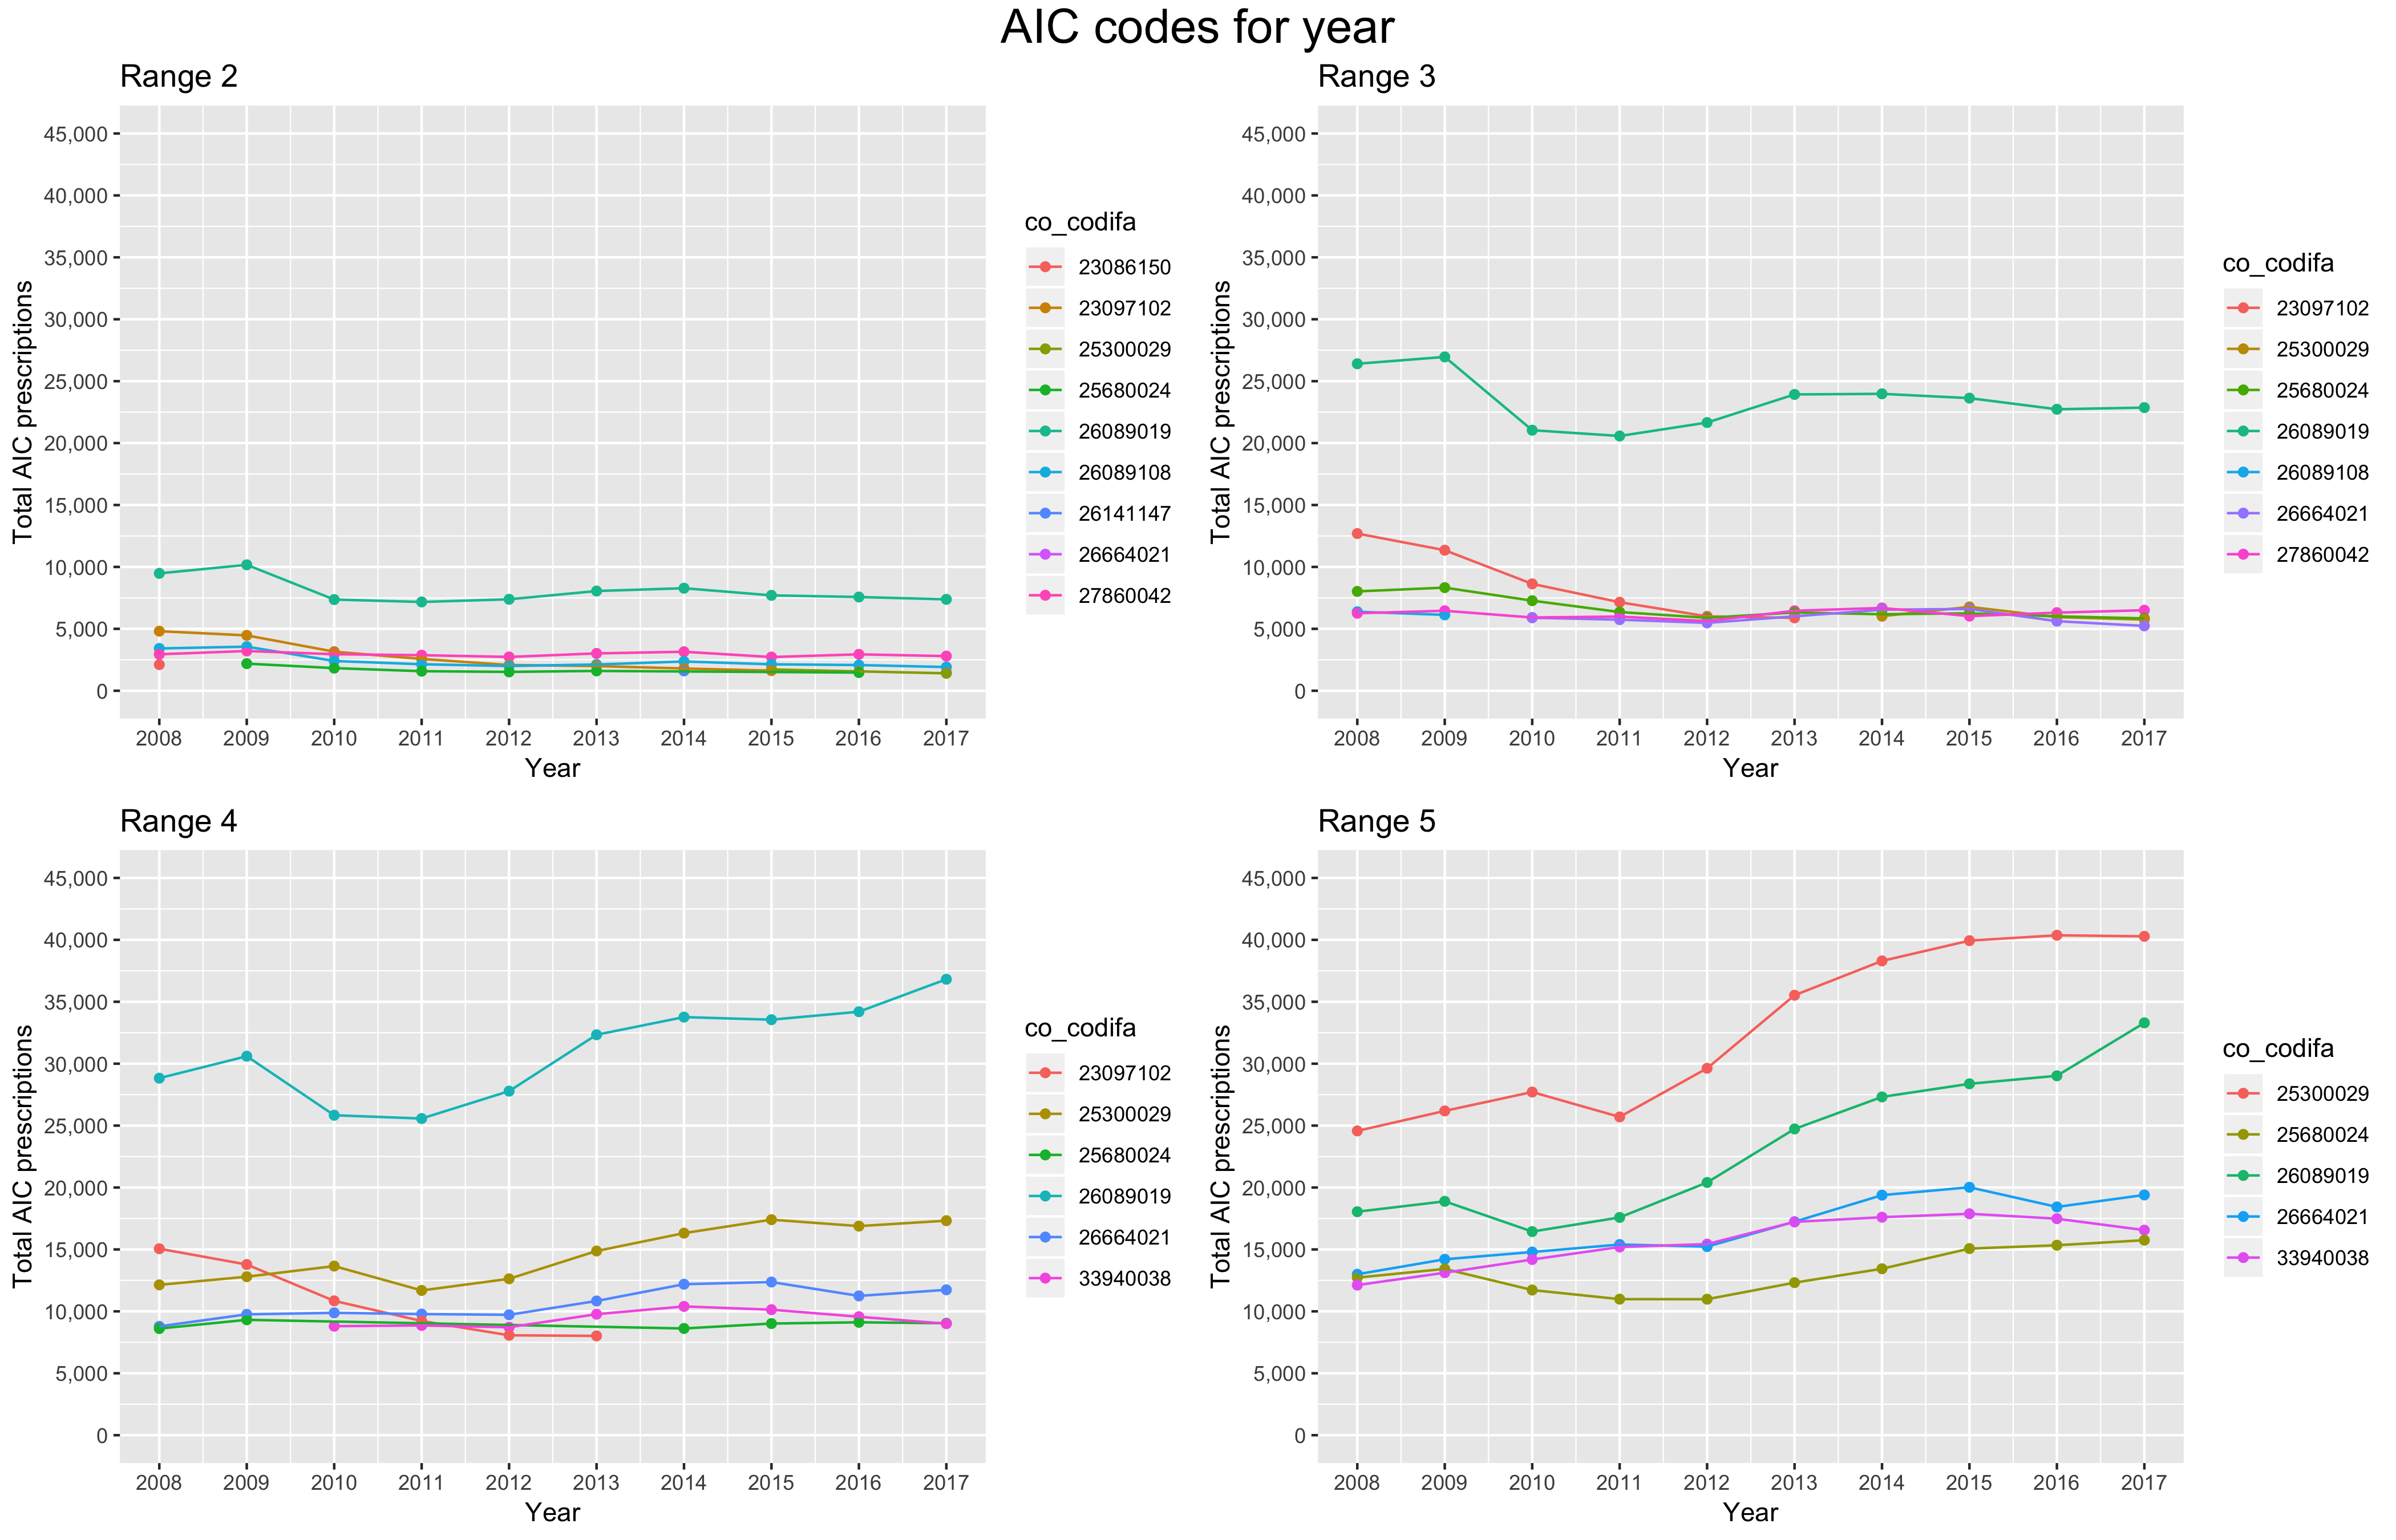
\includegraphics[scale=0.29]{../plots/top_aic_age-year.png}
\end{figure}

\begin{figure}[h]
	\centering
	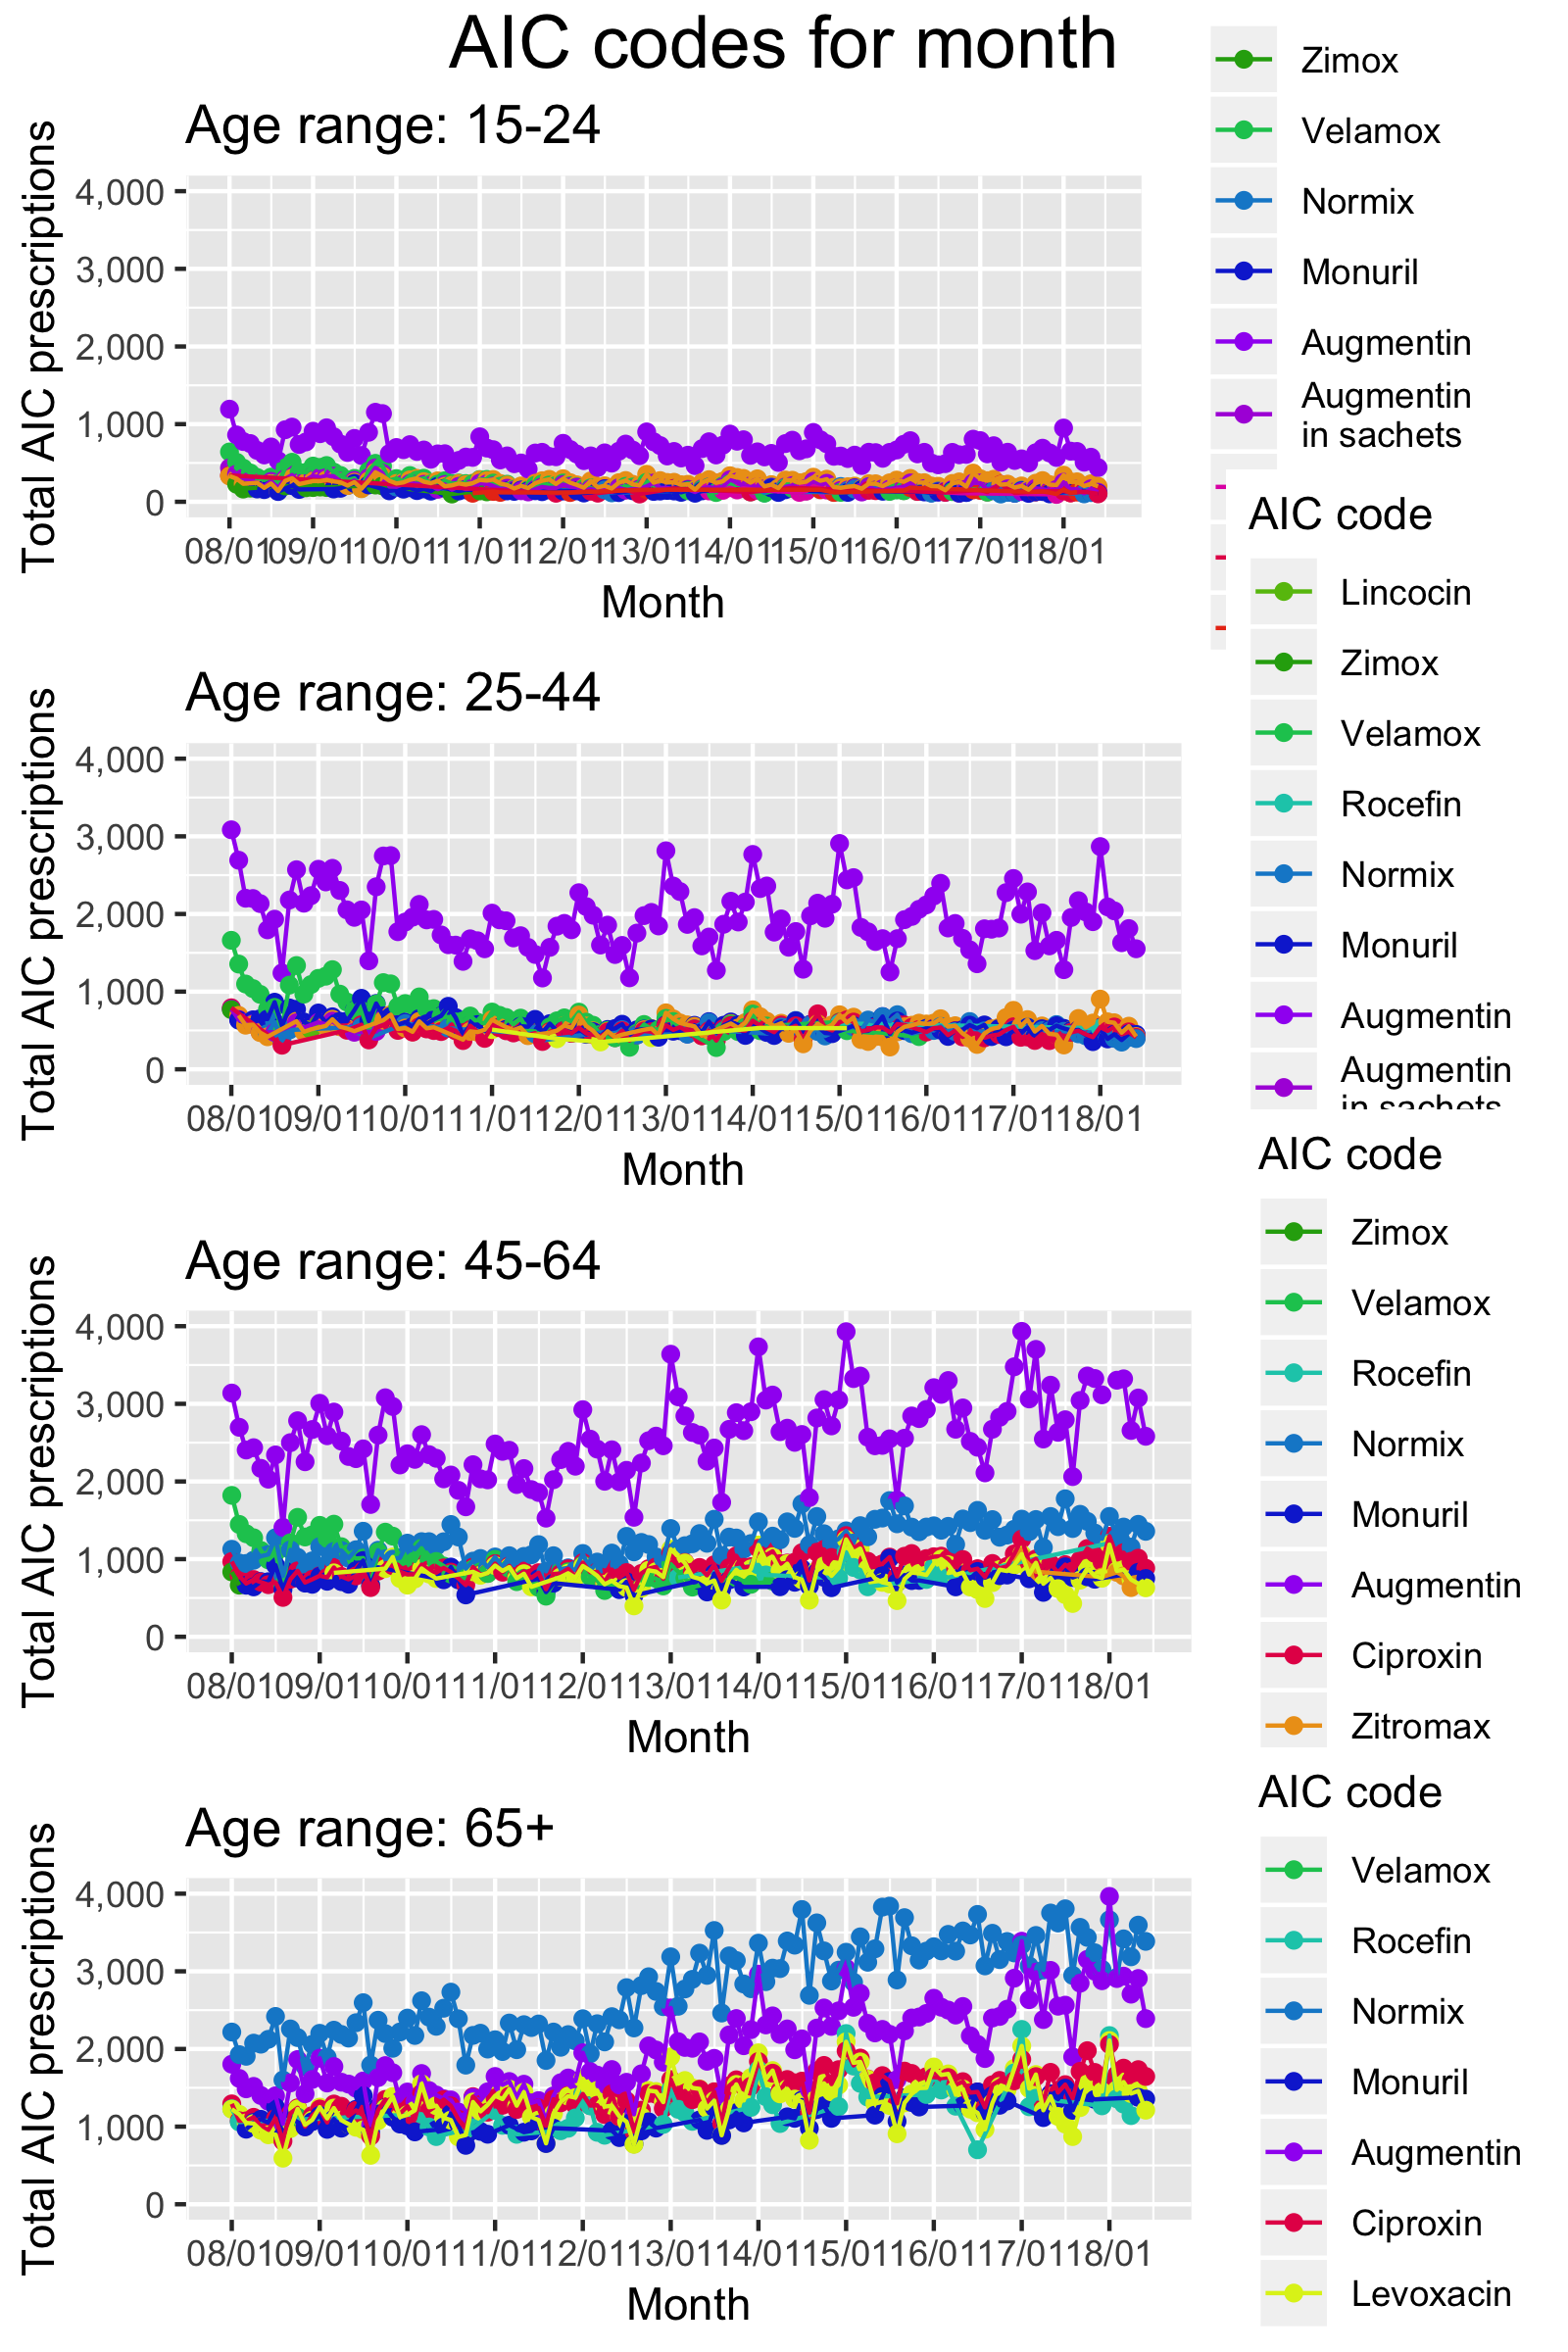
\includegraphics[scale=0.29]{../plots/top_aic_age-month.png}
\end{figure}

\subsection{ATC and AIC correlation}

